\chapter{Desarrollo de Ascension}


El presente capítulo constituye el núcleo técnico de la memoria y describe la implementación detallada de cada subsistema del videojuego \textit{Ascension}. Partiendo del diseño presentado previamente -- requisitos, arquitectura y patrones de diseño --, se documenta cada módulo con sus correspondientes fragmentos de código, explicaciones línea por línea y diagramas de interacción. Al final del capítulo se describen dos sistemas desarrollados pero pendientes de integración completa en el flujo de juego.

El desarrollo de cada subsistema siguió la metodología iterativa e incremental descrita en la introducción. Las secciones de este capítulo presentan el resultado final de cada módulo tras las iteraciones realizadas; al inicio de cada sección se incluye un breve párrafo de \textbf{evolución iterativa} que documenta los cambios de diseño más relevantes que se produjeron durante el proceso de desarrollo, proporcionando trazabilidad entre la metodología adoptada y las decisiones técnicas finales.

\section{Sistema de gestión central}


\textbf{Evolución iterativa.} El sistema de gestión central atravesó tres iteraciones significativas. En la primera versión, el \texttt{GameManager} gestionaba directamente la generación de salas, la aparición de enemigos y la puntuación en una única clase monolítica de más de 500 líneas. La validación funcional reveló que esta concentración de responsabilidades dificultaba la depuración -- un error en la generación de salas afectaba a la lógica de puntuación -- y violaba el principio de responsabilidad única. En la segunda iteración se extrajeron el \texttt{RoomFlowController}, el \texttt{ScoreManager} y el \texttt{DamageBoostManager} como gestores independientes, cada uno con su propio ciclo de vida \textit{Singleton}. La tercera iteración introdujo el sistema de eventos (\texttt{OnGameStateChanged}, \texttt{OnRoomCleared}, \texttt{OnEnemyKilled}) para desacoplar la comunicación entre gestores: en la versión anterior, el \texttt{GameManager} invocaba métodos concretos de cada componente de UI, lo que obligaba a modificar el gestor central cada vez que se añadía un nuevo elemento a la interfaz.

\subsection{GameManager: controlador principal del juego}


El \texttt{GameManager} constituye el componente central del sistema. Implementa el patrón \textit{Singleton} con el objetivo de mantener una única instancia, y gestiona el ciclo de vida completo de una partida mediante una máquina de estados finitos (FSM). Sus responsabilidades incluyen el control de estados del juego, la gestión de progresión (salas completadas, enemigos eliminados), las transiciones entre escenas y la coordinación de los subsistemas.

\textbf{Máquina de estados.} El flujo del juego se modela mediante una enumeración que define los estados válidos:

\begin{lstlisting}
public enum GameState {
    Menu,
    CharacterSelection,
    Playing,
    Paused,
    GameOver,
    Victory
}
\end{lstlisting}


Las transiciones entre estados se gestionan mediante un método centralizado que modifica el estado actual, ajusta la escala de tiempo del juego y notifica a los observadores suscritos:

\begin{lstlisting}
public void ChangeState(GameState newState) {
    if (currentState == newState) return;    // Evita transiciones redundantes
    
    currentState = newState;
    
    switch (newState) {
        case GameState.Playing:
            Time.timeScale = 1f;             // Tiempo normal: fisica y animaciones activas
            isPaused = false;
            break;
        case GameState.Paused:
            Time.timeScale = 0f;             // Detiene la simulacion completa
            isPaused = true;
            break;
        case GameState.GameOver:
        case GameState.Victory:
            Time.timeScale = 0f;             // Congela el juego tras el resultado
            break;
    }
    
    OnGameStateChanged?.Invoke(newState);    // Notifica a todos los suscriptores
}
\end{lstlisting}


Línea por línea:

\begin{itemize}
\item \texttt{if (currentState == newState) return}: previene notificaciones duplicadas si un componente solicita transitar al estado en el que ya se encuentra el juego, lo que evitaría efectos colaterales como reactivar paneles de UI que ya están visibles.
\item \texttt{Time.timeScale = 0f}: detiene toda la simulación dependiente del tiempo escalado (física del \texttt{Rigidbody2D}, animaciones del \texttt{Animator}, corutinas que usen \texttt{WaitForSeconds}). Se seleccionó \texttt{Time.timeScale} frente a la alternativa de desactivar componentes individuales porque proporciona una pausa global con una sola asignación, sin necesidad de iterar sobre todos los objetos activos de la escena.
\item \texttt{OnGameStateChanged?.Invoke(newState)}: emite el evento del patrón \textit{Observer}. El operador \texttt{?.} evita una excepción si ningún componente está suscrito al evento. Los componentes de UI (\texttt{PauseMenu}, \texttt{GameOverScreen}) se suscriben a este evento en su método \texttt{Start()} y reaccionan automáticamente al cambio de estado.
\end{itemize}

\begin{figure}[H]
\begin{center}
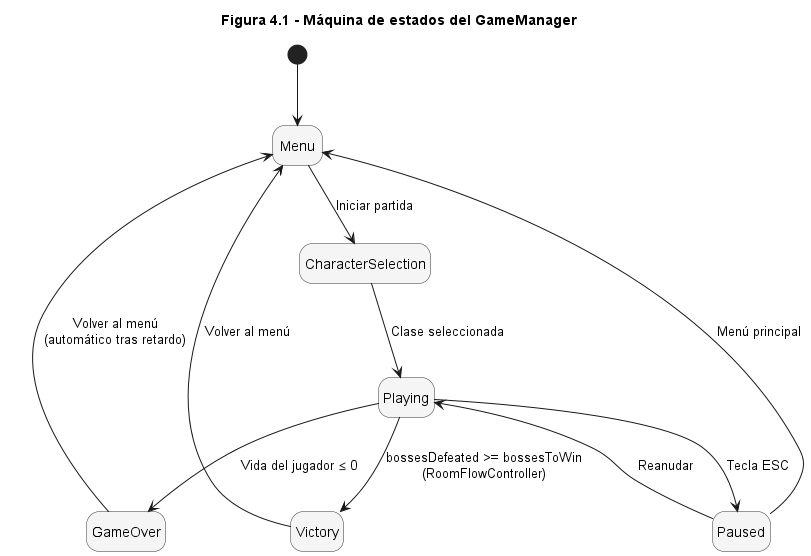
\includegraphics[width=0.95\textwidth,height=0.72\textheight,keepaspectratio]{Figuras/figura4_1_gamemanager_estados.png}
\caption{
Diagrama de estados UML del \texttt{GameManager}. \textit{Elaboración propia.}
}
\label{fig:placeholder-1}
\end{center}
\end{figure}


\textbf{Patrón Singleton.} La inicialización del \textit{Singleton} se realiza en el método \texttt{Awake()}, con el objetivo de que solo exista una instancia del gestor y que esta persista entre cambios de escena:

\begin{lstlisting}
void Awake() {
    if (Instance == null) {
        Instance = this;
        
        if (ScoreManager.Instance == null) {
            new GameObject("ScoreManager").AddComponent<ScoreManager>();
        }
        DontDestroyOnLoad(gameObject);
    } else {
        Destroy(gameObject);
        return;
    }
}
\end{lstlisting}


La comprobación \texttt{if (Instance == null)} previene la creación de instancias duplicadas cuando se vuelve a cargar una escena que contenga un \texttt{GameManager} en su jerarquía. Adicionalmente, si no existe un \texttt{ScoreManager} activo, el \texttt{GameManager} lo crea de forma automática, de forma que el sistema de puntuación esté disponible. La llamada a \texttt{DontDestroyOnLoad} se realiza al final del bloque para que tanto el \texttt{GameManager} como el \texttt{ScoreManager} recién creado persistan entre cambios de escena. Si ya existe una instancia, el duplicado se destruye y se retorna inmediatamente con \texttt{return}.

\textbf{Sistema de eventos.} El \texttt{GameManager} expone tres eventos principales que implementan el patrón \textit{Observer}:

\begin{table}[H]
\begin{center}
\small
\begin{tabular}{|p{0.307\textwidth}|p{0.307\textwidth}|p{0.307\textwidth}|}
\hline
\textbf{Evento} & \textbf{Momento de emisión} & \textbf{Suscriptores típicos} \\ \hline
\texttt{OnGameStateChanged} & Al cambiar el estado del juego & \texttt{PauseMenu}, pantallas de fin de partida, sistemas de UI \\ \hline
\texttt{OnRoomCleared} & Al completar una sala & \texttt{RoomFlowController}, \texttt{ScoreDisplay} \\ \hline
\texttt{OnEnemyKilled} & Al eliminar un enemigo & \texttt{ScoreManager}, contadores de UI \\ \hline
\end{tabular}
\end{center}
\end{table}


\TablaTitulo{Eventos del \texttt{GameManager}.
}

\textbf{Inicio de partida y coordinación entre gestores.} El método \texttt{StartNewRun()} constituye el punto de entrada de cada nueva partida y ejemplifica la coordinación entre los cuatro gestores \textit{Singleton} del sistema. Al iniciar una ejecución, el \texttt{GameManager} reinicia sus propios contadores y delega el reinicio de cada subsistema en el gestor correspondiente:

\begin{lstlisting}
public void StartNewRun() {
    currentLevel = 1;
    roomsCleared = 0;
    enemiesKilled = 0;
    
    RoomFlowController.Instance?.ResetRunProgress();   // Reinicia profundidad de sala y secuencia de jefes
    ScoreManager.Instance?.ResetScore();               // Pone la puntuacion a cero
    DamageBoostManager.Instance?.ResetBoost();          // Elimina bonificaciones de dano residuales
    
    ChangeState(GameState.Playing);                    // Transita a Playing -> Time.timeScale = 1
}
\end{lstlisting}


La secuencia de reinicio sigue un orden específico: primero se reinician los datos del \texttt{GameManager}, después los de cada gestor dependiente y, finalmente, se cambia el estado a \texttt{Playing}. Este orden garantiza que los subsistemas estén en un estado limpio \textit{antes} de que la transición de estado notifique a los suscriptores del evento \texttt{OnGameStateChanged} -- incluida la interfaz de usuario, que al recibir la notificación de estado \texttt{Playing} consulta los contadores, que ya deben estar a cero. Si el cambio de estado se realizase antes de los reinicios, los componentes de UI mostrarían brevemente los datos de la partida anterior.

El siguiente diagrama resume la cadena de coordinación entre gestores al iniciar una nueva partida:

\begin{figure}[H]
\begin{center}
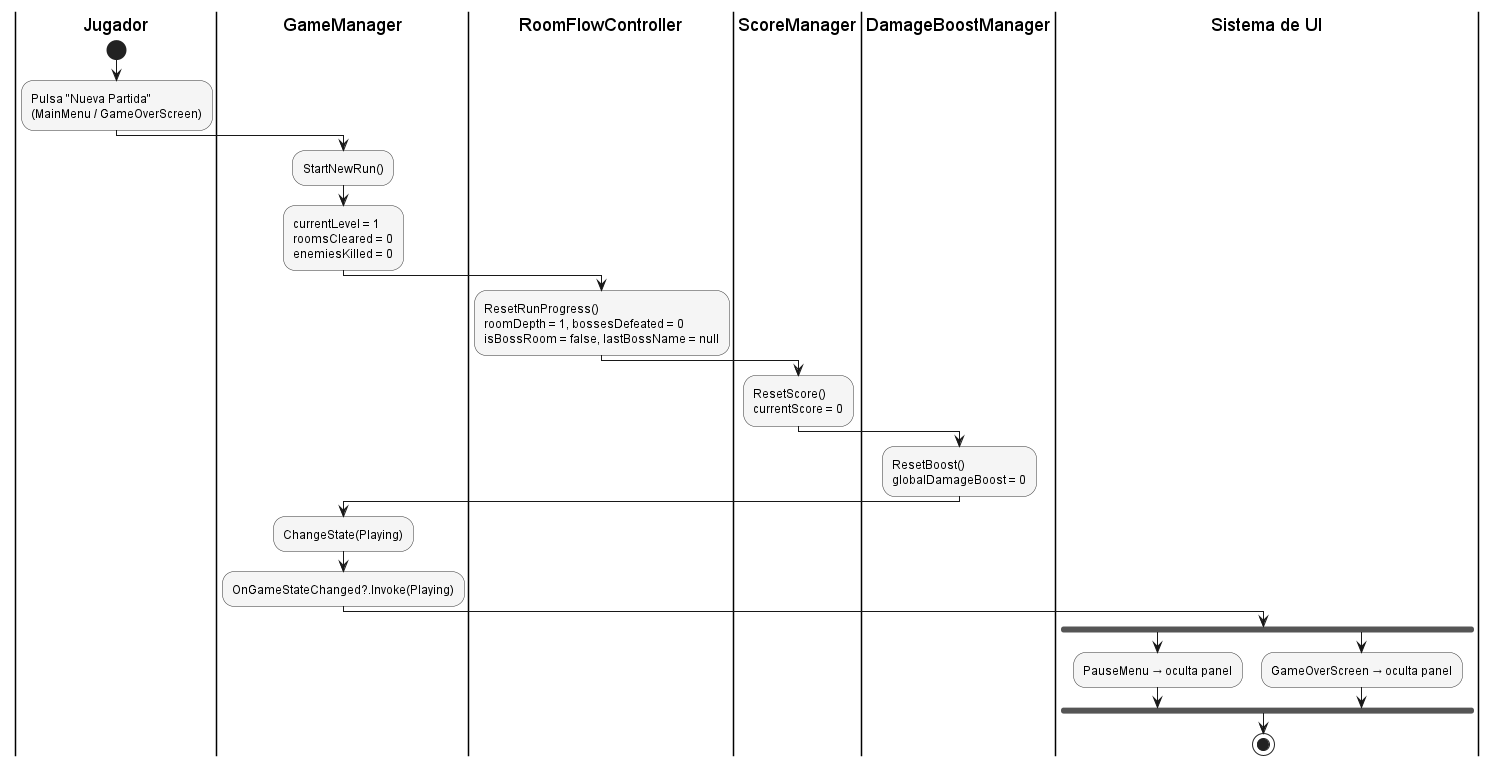
\includegraphics[width=0.95\textwidth,height=0.72\textheight,keepaspectratio]{Figuras/cadena_startnewrun.png}
\caption{
Diagrama de la coordinación entre gestores al iniciar una nueva partida. \textit{Elaboración propia.}
}
\label{fig:placeholder-2}
\end{center}
\end{figure}


\textbf{Sistema de progresión.} La puntuación se calcula según las siguientes reglas: 100 puntos por cada sala completada, una cantidad variable por cada enemigo eliminado (calculada como el daño base del enemigo multiplicado por 5), y una bonificación de 1.000 puntos en caso de completar el juego con victoria.

\textbf{Notificación de sala completada y eliminación de enemigo.} Los métodos \texttt{NotifyRoomCleared()} y \texttt{NotifyEnemyKilled()} completan el ciclo de coordinación entre el \texttt{GameManager} y los subsistemas dependientes:

\begin{lstlisting}
public void NotifyRoomCleared() {
    roomsCleared++;
    ScoreManager.Instance?.Add(100);         // 100 puntos por sala
    OnRoomCleared?.Invoke(roomsCleared);     // Notifica a RoomFlowController y UI
}

public void NotifyEnemyKilled(int scoreValue = 10) {
    enemiesKilled++;
    ScoreManager.Instance?.Add(scoreValue);  // Puntos = dano del enemigo  5
    OnEnemyKilled?.Invoke(enemiesKilled);    // Actualiza contadores de UI
}
\end{lstlisting}


El flujo completo de una sala -- desde la aparición de enemigos hasta la transición a la siguiente sala -- involucra la siguiente cadena de invocaciones entre gestores:

\begin{figure}[H]
\begin{center}
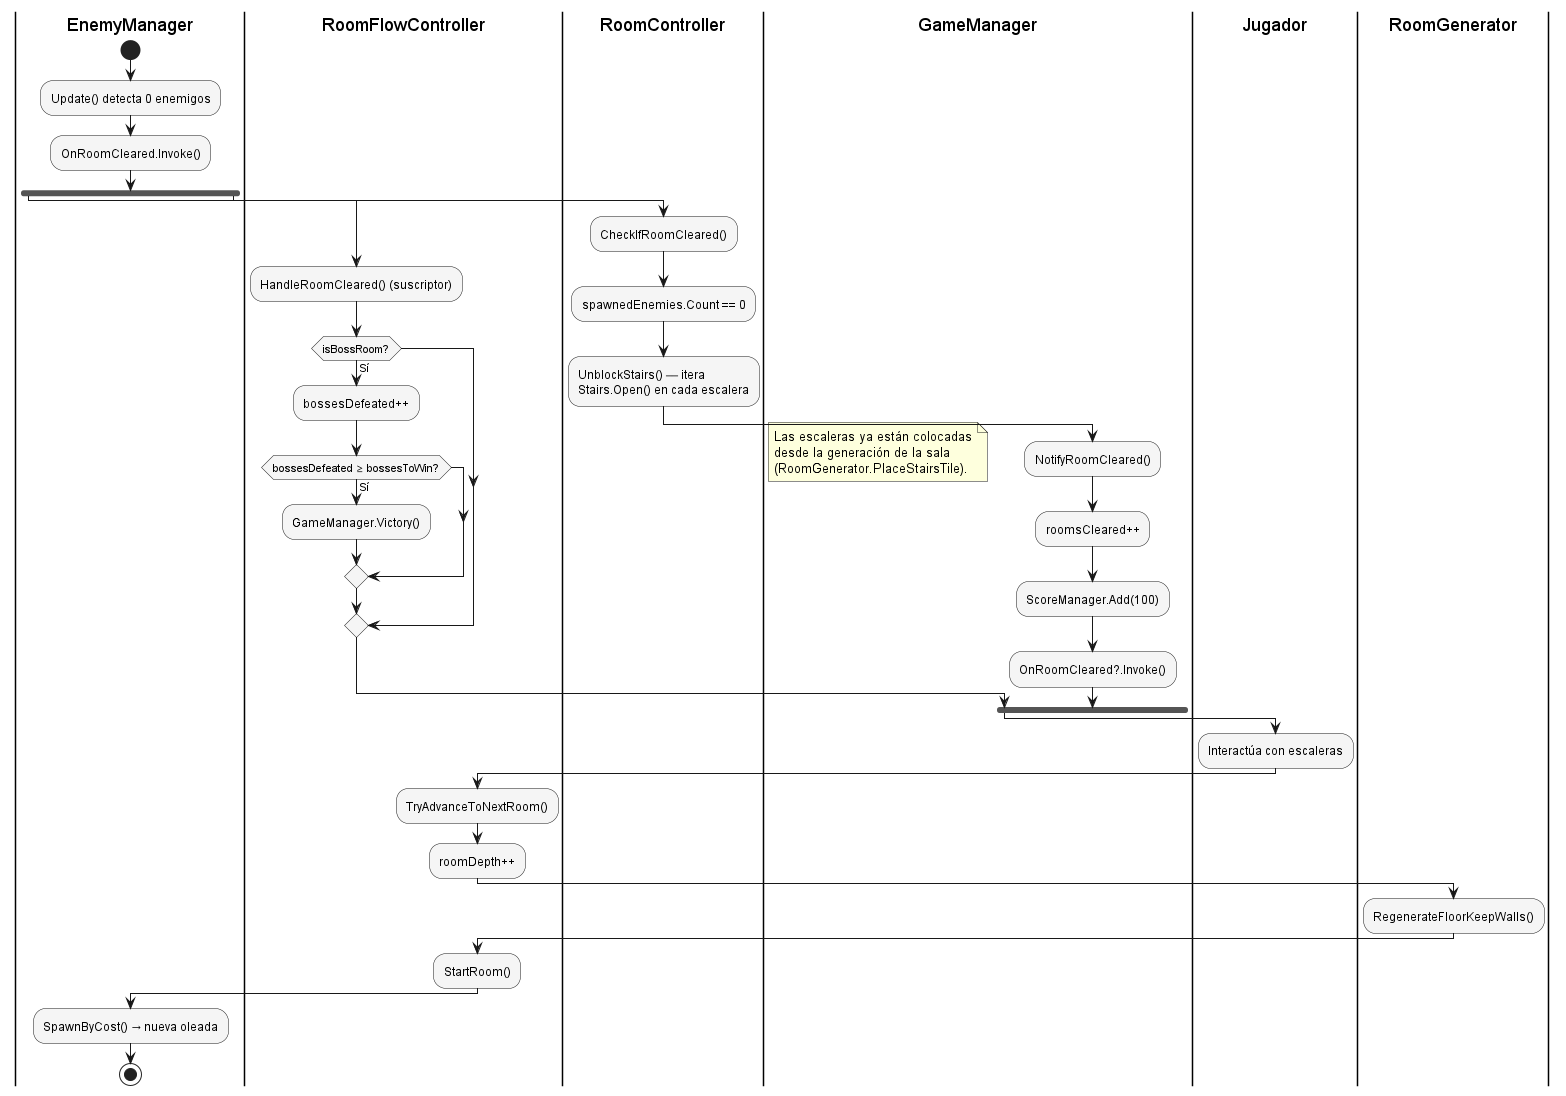
\includegraphics[width=0.95\textwidth,height=0.72\textheight,keepaspectratio]{Figuras/flujo_completar_sala.png}
\caption{
Diagrama del flujo de completar una sala. \textit{Elaboración propia.}
}
\label{fig:placeholder-3}
\end{center}
\end{figure}


\begin{figure}[H]
\begin{center}
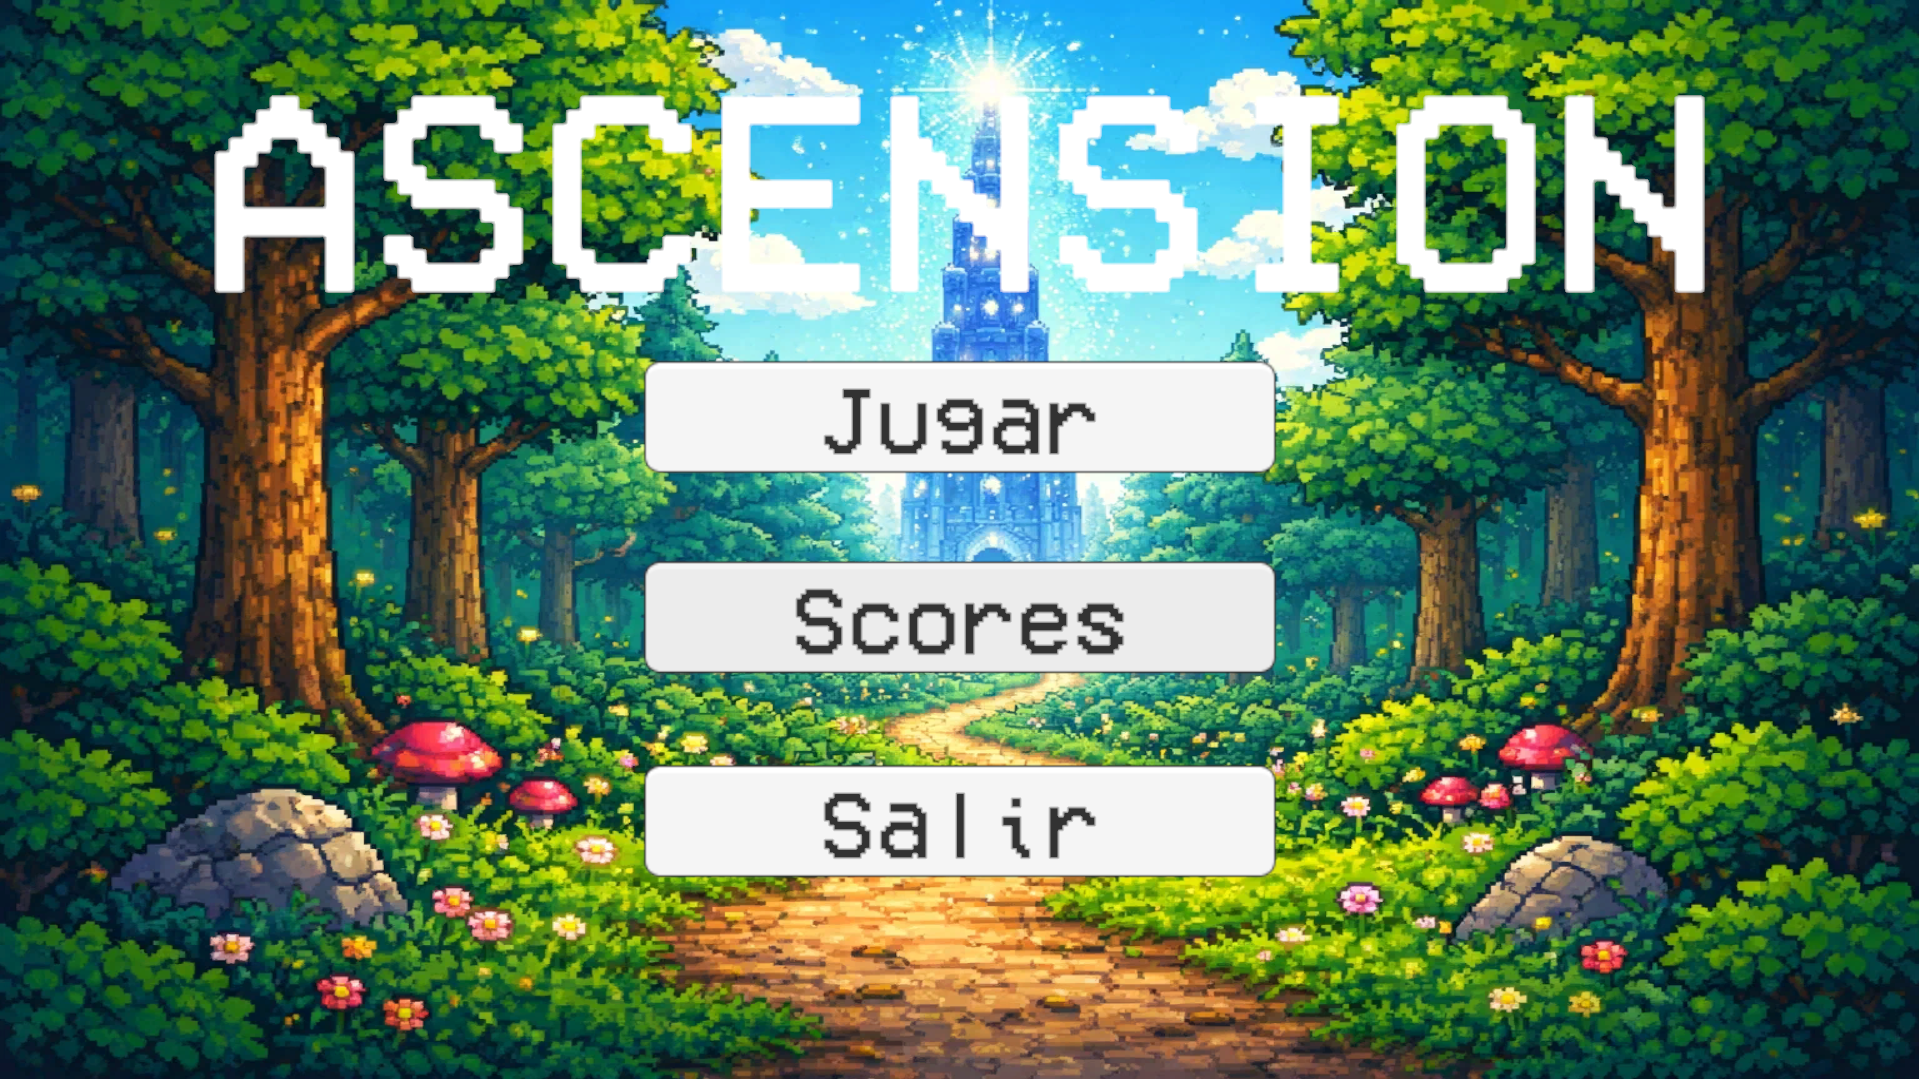
\includegraphics[width=0.9\textwidth]{Figuras/Main_Menu.png}
\caption{Captura de pantalla del menú principal de \textit{Ascension}, mostrando las opciones de nueva partida, tabla de puntuaciones y salir. \textit{Elaboración propia.}}
\label{fig:placeholder-4}
\end{center}
\end{figure}


\subsection{RoomFlowController: control de progresión de salas}


El \texttt{RoomFlowController} gestiona el bucle central de generación y progresión de salas. Su ciclo de funcionamiento se describe mediante el siguiente diagrama:

\begin{figure}[H]
\begin{center}
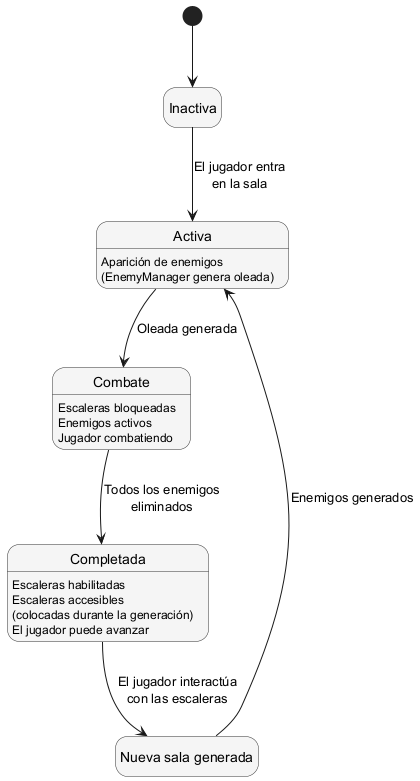
\includegraphics[width=0.95\textwidth,height=0.72\textheight,keepaspectratio]{Figuras/estados_sala.png}
\caption{
Diagrama del ciclo de funcionamiento de generación de salas. \textit{Elaboración propia.}
}
\label{fig:placeholder-5}
\end{center}
\end{figure}


\textbf{Sistema de jefes periódicos.} Cada cinco salas completadas, la siguiente sala contiene un enemigo jefe en lugar de una oleada estándar. En este proyecto, un “jefe” no introduce una IA completamente nueva, sino que se define como una \textbf{variante del enemigo base con atributos incrementados} (\textit{escalado}): mayor tamaño visual (multiplicador de escala de $2{,}4\times$) y mayor resistencia (multiplicador de vida de ocho veces). Este enfoque permite introducir picos de dificultad de forma controlada sin añadir un subsistema adicional de IA de jefes.
\begin{itemize}
\item Jefe 1: Slime verde (francotirador) escalado
\item Jefe 2: Slime rojo (perseguidor) escalado
\item Jefe 3: Slime azul (saltador) escalado
\end{itemize}

\subsection{ScoreManager: sistema de puntuación y persistencia}


El \texttt{ScoreManager} implementa la persistencia de datos de partidas mediante \texttt{PlayerPrefs} y serialización JSON. \texttt{PlayerPrefs} es un mecanismo de almacenamiento local simple (pares clave–valor) proporcionado por Unity, adecuado para guardar preferencias y pequeños volúmenes de datos. La serialización a JSON convierte las estructuras del historial en texto estructurado para poder almacenarlas y recuperarlas de forma consistente entre ejecuciones del juego. Cada entrada del historial almacena la siguiente información:

\begin{lstlisting}
public class ScoreEntry {
    public long utcTicks;        // Marca de tiempo
    public int score;            // Puntuacion final
    public int roomsCleared;     // Salas completadas
    public int enemiesKilled;    // Enemigos eliminados
    public string playerClass;   // Clase utilizada
    public string result;        // "Victory" o "GameOver"
}
\end{lstlisting}


El historial se limita a un máximo de 30 entradas, realizando limpieza automática de las entradas más antiguas cuando se alcanza este límite. Los datos se persisten entre sesiones de juego mediante su serialización a formato JSON y su almacenamiento en \texttt{PlayerPrefs}.



\section{Sistema del jugador}


\textbf{Evolución iterativa.} El sistema del jugador experimentó ajustes relevantes durante el desarrollo. La primera implementación del movimiento utilizaba \texttt{GetAxis} (con suavizado) en lugar de \texttt{GetAxisRaw}, lo que generaba una latencia perceptible entre la pulsación de tecla y el inicio del movimiento; las sesiones de juego revelaron que esta latencia era inadecuada para un \textit{roguelike} de acción, y se sustituyó por \texttt{GetAxisRaw}. El sistema de esquiva (\textit{roll}) se incorporó en una iteración posterior a la implementación del sistema de enemigos: las primeras pruebas de combate demostraron que el jugador carecía de opciones defensivas activas, ya que la única forma de evitar daño era el movimiento. La invulnerabilidad post-daño (parpadeo a 12 Hz) se añadió tras detectar que los enemigos podían infligir varios impactos en fotogramas consecutivos, resultando en muertes instantáneas que el jugador percibía como injustas.

\subsection{PlayerController: control de movimiento}


El \texttt{PlayerController} gestiona el movimiento del personaje, la habilidad de esquiva y la inicialización basada en la clase seleccionada. El sistema de movimiento soporta ocho direcciones y normaliza el vector resultante para evitar que el movimiento diagonal sea más rápido que el movimiento en ejes cardinales:

\begin{lstlisting}
void Update() {
    if (isRolling) return;
    float hor = Input.GetAxisRaw("Horizontal");
    float ver = Input.GetAxisRaw("Vertical");
    velocity = new Vector3(hor, ver, 0).normalized * speed;
    if (canRoll && Input.GetKeyDown(rollKey)) {
        Vector2 rollDir = new Vector2(hor, ver).normalized;
        StartCoroutine(DoRoll(rollDir));
    }
}

void FixedUpdate() {
    if (!isRolling && rigidbody != null) {
        rigidbody.MovePosition(rigidbody.position + (Vector2)(velocity * Time.fixedDeltaTime));
    }
}
\end{lstlisting}


Línea por línea:

\begin{itemize}
\item \textbf{Línea 1:} Si el jugador está ejecutando una esquiva, se ignora toda la entrada de movimiento; el \textit{roll} tiene su propia lógica de velocidad gestionada por la corutina.
\item \textbf{Líneas 2-3:} \texttt{GetAxisRaw} devuelve -1, 0 o 1 sin suavizado de transición, lo que produce un movimiento inmediato y responsivo. Se seleccionó \texttt{GetAxisRaw} frente a \texttt{GetAxis} porque este último aplica un suavizado temporal que introduce latencia perceptible entre la pulsación de tecla y el movimiento, inadecuado para un \textit{roguelike} de acción en tiempo real donde la precisión de movimiento es crítica.
\item \textbf{Línea 4:} \texttt{.normalized} convierte el vector a magnitud 1 antes de multiplicar por \texttt{speed}. Esta normalización resuelve un problema clásico de los videojuegos 2D: sin ella, el movimiento diagonal (por ejemplo, W+D) tendría magnitud $\sqrt{2} \approx 1{,}41$, lo que haría al personaje un 41 \% más rápido en diagonal que en ejes cardinales.
\item \textbf{Líneas 5-7:} La esquiva solo se activa si el jugador puede esquivar (\texttt{canRoll}) y si la tecla se pulsa (\texttt{GetKeyDown}, no \texttt{GetKey}). La dirección del \textit{roll} se calcula a partir de la entrada actual, y se inicia la corutina \texttt{DoRoll(rollDir)} que gestiona la velocidad, la invulnerabilidad y la travesía de colisiones.
\item \textbf{Líneas 8-10:} La aplicación de movimiento se realiza en \texttt{FixedUpdate()} mediante \texttt{MovePosition}, que desplaza al jugador basándose en la velocidad calculada multiplicada por \texttt{fixedDeltaTime}. Se utiliza \texttt{MovePosition} en lugar de asignar \texttt{linearVelocity} porque este método respeta la interpolación del \texttt{Rigidbody2D} y produce un movimiento más suave. \texttt{FixedUpdate()} se ejecuta a una frecuencia fija (50 Hz de forma predeterminada) independiente de la tasa de fotogramas.
\end{itemize}

\textbf{Inicialización basada en clase.} Al instanciar al jugador, el \texttt{PlayerController} recibe un \textit{ScriptableObject} de tipo \texttt{PlayerClass} que define las estadísticas iniciales del personaje y el arma con la que comienza la partida:

\begin{lstlisting}
public void Initialize() {
    baseSpeed = playerClass.speed;
    speed = baseSpeed;
    
    // Instanciar arma inicial
    GameObject weaponInstance = Instantiate(
        playerClass.startingWeaponData.weaponPrefab,
        transform.position,
        Quaternion.identity,
        transform
    );
    
    // Inicializar script del arma
    Weapon weaponScript = weaponInstance.GetComponent<Weapon>();
    weaponScript.weaponData = playerClass.startingWeaponData;
    weaponScript.Initialize();
}
\end{lstlisting}


Este diseño permite añadir nuevas clases de personaje sin modificar el código del \textit{controller}, ya que toda la configuración se define en activos de tipo \textit{ScriptableObject} editables desde el inspector de Unity.

\textbf{Sistema de esquiva (\textit{roll}).} La mecánica de esquiva se implementa mediante una corutina que aplica un multiplicador de velocidad temporal, activa la invulnerabilidad del jugador y desactiva las colisiones con enemigos y proyectiles durante un periodo configurable. Al finalizar la esquiva, el sistema restaura los valores originales de velocidad, vulnerabilidad y colisiones:

\begin{figure}[H]
\begin{center}
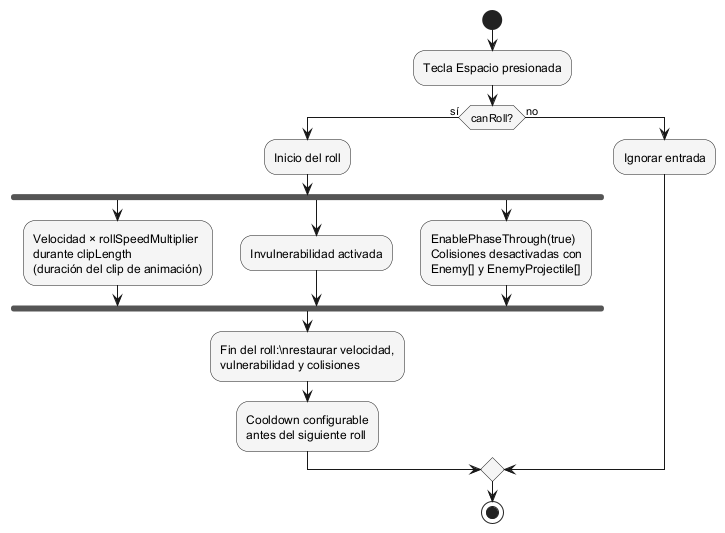
\includegraphics[width=0.95\textwidth,height=0.72\textheight,keepaspectratio]{Figuras/mecanica_esquiva.png}
\caption{
Diagrama del funcionamiento de la esquiva. \textit{Elaboración propia.}
}
\label{fig:placeholder-6}
\end{center}
\end{figure}


\textbf{Travesía de colisiones (\textit{phase-through}).} Durante la esquiva, el jugador atraviesa a los enemigos y sus proyectiles. El método \texttt{EnablePhaseThrough} utiliza \texttt{Physics2D.IgnoreCollision} de Unity para desactivar selectivamente las colisiones entre el colisionador del jugador y los de cada enemigo y proyectil enemigo activos en la escena:

\begin{lstlisting}
private void EnablePhaseThrough(bool enable) {
    Collider2D playerCollider = GetComponent<Collider2D>();
    if (playerCollider == null) return;
    
    Enemy[] enemies = FindObjectsByType<Enemy>(FindObjectsSortMode.None);
    foreach (Enemy enemy in enemies) {
        if (enemy != null) {
            Collider2D enemyCollider = enemy.GetComponent<Collider2D>();
            if (enemyCollider != null)
                Physics2D.IgnoreCollision(playerCollider, enemyCollider, enable);
        }
    }
    
    EnemyProjectile[] projectiles = FindObjectsByType<EnemyProjectile>(FindObjectsSortMode.None);
    foreach (EnemyProjectile proj in projectiles) {
        if (proj != null) {
            Collider2D projCollider = proj.GetComponent<Collider2D>();
            if (projCollider != null)
                Physics2D.IgnoreCollision(playerCollider, projCollider, enable);
        }
    }
}
\end{lstlisting}


Se seleccionó \texttt{Physics2D.IgnoreCollision} frente a la alternativa de cambiar la capa del jugador (\textit{layer}) durante la esquiva, porque el cambio de capa afectaría a todas las interacciones del jugador (incluidas paredes y tiles), mientras que \texttt{IgnoreCollision} permite desactivar selectivamente solo las colisiones con enemigos y proyectiles, manteniendo intactas las colisiones con el entorno.

\subsection{PlayerHealth: sistema de vida}


El \texttt{PlayerHealth} gestiona los puntos de vida del jugador, el sistema de invulnerabilidad temporal tras recibir daño y la detección de muerte. El método principal de recepción de daño ilustra el flujo completo:

\begin{lstlisting}
public void TakeDamage(int amount) {
    if (isInvulnerable || (playerController != null && playerController.IsInvulnerable()))
        return;
    
    currentHealth -= amount;
    currentHealth = Mathf.Clamp(currentHealth, 0, maxHealth);
    
    UpdateHearts();
    
    if (currentHealth <= 0) {
        Die();
    } else {
        if (damageCoroutine != null)
            StopCoroutine(damageCoroutine);
        damageCoroutine = StartCoroutine(DamageInvulnerabilityCoroutine());
    }
}
\end{lstlisting}


La verificación inicial comprueba si el jugador se encuentra en estado de invulnerabilidad, ya sea por haber recibido daño previamente (invulnerabilidad temporal) o por estar ejecutando una esquiva; la comprobación \texttt{playerController != null} previene errores si la referencia aún no está inicializada. La función \texttt{Mathf.Clamp} evita que la vida descienda por debajo de cero o exceda el máximo. Tras actualizar la representación visual de los corazones, se evalúa si el jugador ha muerto; en caso contrario, se cancela cualquier corutina de parpadeo en curso (\texttt{damageCoroutine}) antes de iniciar una nueva, evitando conflictos visuales cuando el jugador recibe impactos consecutivos.

\textbf{Efecto visual de parpadeo.} Durante el periodo de invulnerabilidad, el sprite del jugador parpadea alternando entre su color original y blanco, y opcionalmente alternando su visibilidad, a una frecuencia configurable (de forma predeterminada, doce Hz). Si existe una corutina de parpadeo anterior en curso, se cancela antes de iniciar la nueva para evitar conflictos:

\begin{lstlisting}
private IEnumerator DamageInvulnerabilityCoroutine() {
    isInvulnerable = true;

    if (spriteRenderers == null || spriteRenderers.Length == 0)
        CacheSpriteRenderers();

    float end = Time.time + Mathf.Max(0f, invulnerableTime);
    float blinkPeriod = blinkFrequencyHz > 0f ? (1f / blinkFrequencyHz) : 0.1f;
    float nextToggle = 0f;
    bool white = true;
    bool visible = true;

    while (Time.time < end) {
        if (Time.time >= nextToggle) {
            nextToggle = Time.time + blinkPeriod;
            white = !white;
            visible = !visible;
        }

        for (int i = 0; i < spriteRenderers.Length; i++) {
            var sr = spriteRenderers[i];
            if (sr == null) continue;
            sr.enabled = visibilityBlinkOnDamage ? visible : true;
            sr.color = white ? Color.white : originalColors[i];
        }

        yield return null;
    }

    for (int i = 0; i < spriteRenderers.Length; i++) {
        if (spriteRenderers[i] == null) continue;
        spriteRenderers[i].color = originalColors[i];
        spriteRenderers[i].enabled = true;
    }

    isInvulnerable = false;
    damageCoroutine = null;
}
\end{lstlisting}


La instrucción \texttt{yield return null} cede la ejecución hasta el siguiente fotograma sin bloquear el hilo principal del juego. El final del efecto se controla comparando \texttt{Time.time} (tiempo global del juego) con el instante \texttt{end}, lo que permite que la duración de la invulnerabilidad sea consistente independientemente de la tasa de fotogramas.

El cambio de color y visibilidad se aplica a todos los \texttt{SpriteRenderer} del jugador (incluidos los de sus objetos hijos, almacenados en caché por \texttt{CacheSpriteRenderers()}) para que el parpadeo afecte al personaje completo. La variable \texttt{visibilityBlinkOnDamage} permite alternar no solo el color, sino también la visibilidad (\texttt{sr.enabled}) de cada renderer, produciendo un efecto de parpadeo más notorio. Al finalizar la corutina, se restablece el estado original de todos los renderers y se marca \texttt{damageCoroutine = null} para permitir la gestión correcta de corutinas superpuestas.

\subsubsection{Diagrama del ciclo de vida del jugador}


El ciclo de vida del jugador integra los subsistemas de movimiento (\texttt{PlayerController}), vida (\texttt{PlayerHealth}) y esquiva, atravesando los siguientes estados durante una partida:

\begin{figure}[H]
\begin{center}
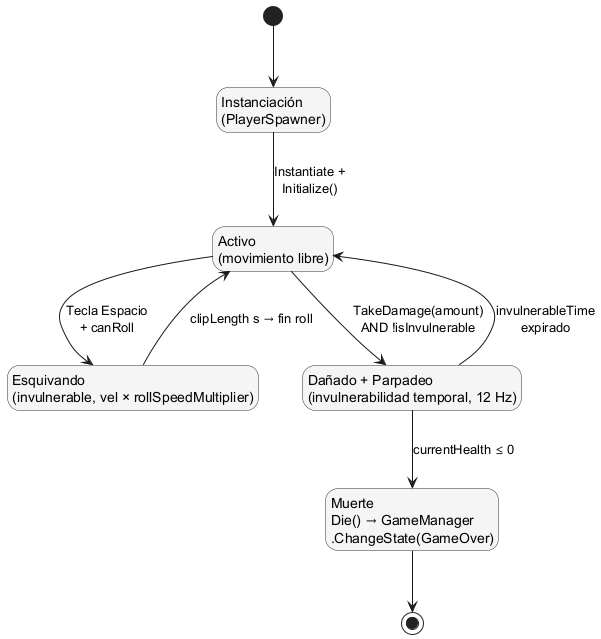
\includegraphics[width=0.95\textwidth,height=0.72\textheight,keepaspectratio]{Figuras/ciclo_vida_jugador.png}
\caption{
Ciclo de vida del jugador. \textit{Elaboración propia.}
}
\label{fig:placeholder-7}
\end{center}
\end{figure}


Este diagrama muestra que el jugador solo puede recibir daño en el estado \textbf{Activo} (ni durante la esquiva ni durante la invulnerabilidad post-daño), lo que proporciona dos mecanismos de protección distintos: uno proactivo (esquiva voluntaria) y otro reactivo (invulnerabilidad automática tras daño). Cuando la vida alcanza cero, se ejecuta un parpadeo rojo rápido (cinco alternancias rojo/blanco a 0,08 s por cambio, duración total de 0,8 s) que proporciona retroalimentación visual de muerte antes de notificar al \texttt{GameManager} para que transite al estado \texttt{GameOver}, ejemplificando la interacción \textit{Observer} + \textit{State Machine} descrita en el capítulo de diseño.

\subsection{PlayerSpawner: instanciación del jugador}


El \texttt{PlayerSpawner} se encarga de instanciar al jugador al inicio de la escena de juego, aplicando la clase seleccionada en la escena anterior:

\begin{lstlisting}
void Start() {
    if (ClassSelectionManager.SelectedClass == null) {
        Debug.LogError("No se ha seleccionado ninguna clase.");
        SceneManager.LoadScene("ClassSelection");
        return;
    }
    
    GameObject player = Instantiate(
        playerPrefab, 
        spawnPoint.position, 
        Quaternion.identity
    );
    
    var controller = player.GetComponent<PlayerController>();
    controller.playerClass = ClassSelectionManager.SelectedClass;
    controller.Initialize();
}
\end{lstlisting}


Si el jugador accede a la escena de juego sin haber seleccionado una clase -- por ejemplo, durante la depuración --, el sistema detecta esta situación y redirige automáticamente a la escena de selección.

\subsection{PlayerClass: datos de configuración mediante \textit{ScriptableObjects}}


Los datos de cada clase de personaje se definen mediante un \textit{ScriptableObject}. Se seleccionó este mecanismo frente a dos alternativas: (a) codificar las estadísticas directamente en variables del \texttt{PlayerController}, lo que obligaría a duplicar y recompilar el script para cada combinación de parámetros; y (b) cargar los datos desde un fichero externo (JSON o XML), lo que añadiría lógica de lectura, deserialización y validación sin integración con el inspector de Unity.

El \textit{ScriptableObject} resuelve ambos problemas: es un activo nativo del proyecto que se edita directamente desde el inspector, se serializa automáticamente con el proyecto, y se vincula al \texttt{PlayerController} mediante una referencia en el campo \texttt{playerClass}. Esta decisión tiene una implicación arquitectónica directa: para añadir una nueva clase de personaje, basta con crear un nuevo activo de tipo \texttt{PlayerClass} desde el menú del editor (\texttt{Roguelike/PlayerClass}), configurar sus estadísticas y asignarle un arma inicial, sin modificar una sola línea del código del \texttt{PlayerController}.

\begin{lstlisting}
[CreateAssetMenu(fileName = "PlayerClass", menuName = "Roguelike/PlayerClass")]
public class PlayerClass : ScriptableObject {
    public string className;        // Nombre visible de la clase (p. ej., "Guerrero")
    public int maxHealth = 5;       // Puntos de vida maximos
    public float speed = 32f;       // Velocidad base en unidades/segundo
    public WeaponData startingWeaponData;  // Referencia al arma inicial (otro ScriptableObject)
}
\end{lstlisting}


Línea por línea:

\begin{itemize}
\item \texttt{[CreateAssetMenu(...)]}: atributo de Unity que añade una entrada al menú contextual del editor, permitiendo crear instancias de este \textit{ScriptableObject} directamente desde \texttt{Assets > Create > Roguelike > PlayerClass}.
\item \texttt{className}: cadena que identifica la clase en la interfaz de usuario (pantalla de selección y estadísticas finales).
\item \texttt{maxHealth = 5}: valor predeterminado que diferencia las clases; el guerrero podría tener 7 y el mago 3.
\item \texttt{speed = 32f}: velocidad base en unidades del mundo por segundo; a 16 PPU (píxeles por unidad), equivale a 512 píxeles por segundo.
\item \texttt{startingWeaponData}: referencia a otro \textit{ScriptableObject} (\texttt{WeaponData}) que define el arma con la que la clase comienza la partida. Esta composición de \textit{ScriptableObjects} permite que la misma arma pueda reutilizarse en múltiples clases sin duplicar datos.
\end{itemize}

\section{Sistema de enemigos}


\textbf{Evolución iterativa.} El sistema de enemigos fue el subsistema que más iteraciones requirió. Inicialmente, cada tipo de enemigo se implementó como una clase independiente sin herencia compartida, lo que provocó duplicación de la lógica de vida, daño y muerte en tres archivos. La refactorización hacia la jerarquía con \textit{Template Method} (clase base \texttt{Enemy} + subclases) se realizó en la cuarta iteración del módulo. El sistema de periodos de gracia (\texttt{contactDamageGraceSeconds}, \texttt{aiGraceSeconds}) se descubrió durante las pruebas de juego: sin este mecanismo, los enemigos dañaban al jugador en el fotograma de aparición. El limitador de velocidad (\texttt{CapToPlayerSpeed}) surgió de la misma forma: el SlimeGreen en estado de huida se movía más rápido que el jugador, haciendo imposible la persecución. Ambos mecanismos se integraron en la clase base \texttt{Enemy} para que todos los tipos de enemigo los heredasen automáticamente.

\subsection{Enemy: clase base y patrón \textit{Template Method}}


La clase \texttt{Enemy} define el comportamiento base compartido por todos los tipos de enemigo del juego. Se seleccionó el patrón \textit{Template Method} frente a la alternativa de implementar cada enemigo como una clase independiente sin herencia. Esta alternativa se descartó porque los tres tipos de enemigo comparten un núcleo de funcionalidad significativo: gestión de puntos de vida (recepción de daño, muerte), periodos de gracia tras la aparición, interacción con tiles de velocidad, detección de contacto con el jugador y notificación al \texttt{GameManager} al morir. Duplicar esta lógica en tres clases independientes habría generado aproximadamente 180 líneas de código redundante y habría introducido riesgo de inconsistencias: si se modificase la lógica de daño en un tipo de enemigo pero no en los demás, se producirían discrepancias difíciles de detectar.

El \textit{Template Method} resuelve este problema: la clase base \texttt{Enemy} define el esqueleto de comportamiento común, y cada subclase sobrescribe exclusivamente el método \texttt{Update()} para definir su IA específica.

\textbf{Sistema de gracia al aparecer.} Para evitar que los enemigos ataquen al jugador inmediatamente tras aparecer -- lo que resultaría en una experiencia injusta --, se implementa un sistema de periodos de gracia:

\begin{lstlisting}
[SerializeField] private float contactDamageGraceSeconds = 0.75f;
[SerializeField] private float aiGraceSeconds = 0.75f;

protected bool IsAIEnabled => Time.time >= aiEnabledTime;
\end{lstlisting}


En este contexto, \texttt{Time.time} representa el tiempo transcurrido desde el inicio de la ejecución del juego. La IA se habilita cuando dicho tiempo supera un instante programado (\texttt{aiEnabledTime}), de modo que el enemigo “espera” un breve intervalo antes de comenzar a actuar.

Durante los primeros 0,75 segundos tras su aparición, el enemigo no puede infligir daño por contacto ni ejecutar su lógica de inteligencia artificial. Este intervalo proporciona al jugador una ventana de reacción justa.

\textbf{Interacción con tiles de velocidad.} Los enemigos, al igual que el jugador, se ven afectados por los tiles de velocidad del suelo:

\begin{lstlisting}
public void SetTileSpeedMultiplier(float multiplier) {
    tileSpeedMultiplier = Mathf.Clamp(multiplier, 0.1f, 5f);
}
\end{lstlisting}


Esta mecánica añade profundidad táctica al combate, ya que el jugador puede utilizar las zonas de lodo para ralentizar a los enemigos perseguidores o las zonas de hielo para alejarse rápidamente.

\textbf{Sistema de muerte.} Al alcanzar cero puntos de vida, el enemigo notifica al \texttt{GameManager} para el cálculo de puntuación y ejecuta un parpadeo rojo de retroalimentación visual antes de destruirse:

\begin{lstlisting}
protected virtual void Die() {
    if (isDead) return;
    isDead = true;

    if (rb != null) {
        rb.linearVelocity = Vector2.zero;
        rb.bodyType = RigidbodyType2D.Kinematic;
    }
    if (animator != null)
        animator.enabled = false;
    
    if (GameManager.Instance != null) {
        int scoreValue = enemyData != null ? enemyData.damage * 5 : 10;
        GameManager.Instance.NotifyEnemyKilled(scoreValue);
    }

    StartCoroutine(DeathBlinkCoroutine());
}

private IEnumerator DeathBlinkCoroutine() {
    int blinks = 4;
    float interval = 0.08f;

    for (int i = 0; i < blinks; i++) {
        SetSpriteRenderersColor(Color.red);
        yield return new WaitForSeconds(interval);
        SetSpriteRenderersColor(Color.white);
        yield return new WaitForSeconds(interval);
    }

    if (animator != null && animator.runtimeAnimatorController != null && hasAnimDieTrigger) {
        animator.enabled = true;
        animator.SetTrigger("Die");
        Destroy(gameObject, 0.5f);
    } else {
        Destroy(gameObject);
    }
}
\end{lstlisting}


Antes de notificar al \texttt{GameManager}, el método \texttt{Die()} congela al enemigo: se anula la velocidad del \texttt{Rigidbody2D} y se cambia su tipo a \texttt{Kinematic} para impedir que la física lo desplace (incluido el \textit{dash} del SlimeBlue, cuyo \texttt{FixedUpdate} sigue asignando velocidad mientras \texttt{isDashing} sea verdadero). Además, se desactiva el \texttt{Animator} para que el sprite quede estático mirando hacia la última dirección, evitando que la animación de movimiento continúe durante el parpadeo. La corutina \texttt{DeathBlinkCoroutine()} alterna el color de todos los \texttt{SpriteRenderer} entre rojo y blanco cuatro veces (intervalo de 0,08 s por cambio, duración total de 0,64 s), proporcionando retroalimentación visual inmediata de eliminación. Tras el parpadeo, si el \texttt{Animator} dispone de un trigger \texttt{Die}, se reactiva para reproducir la animación de muerte y el objeto se destruye tras 0,5 s; en caso contrario, se destruye inmediatamente.

\textbf{Daño por contacto.} Los enemigos infligen daño continuo al jugador mientras permanecen en contacto con él, verificado mediante \texttt{OnCollisionStay2D}. El sistema respeta tanto el periodo de gracia al aparecer como el estado de esquiva del jugador:

\begin{lstlisting}
protected virtual void OnCollisionStay2D(Collision2D collision) {
    if (isDead) return;
    
    if (collision.gameObject.CompareTag("Player")) {
        PlayerController pc = collision.gameObject.GetComponent<PlayerController>();
        if (pc != null && pc.IsRolling) return;          // Sin dano durante roll
        
        if (Time.time < contactDamageEnabledTime) return; // Periodo de gracia
        
        if (Time.time >= lastDamageTime + damageRate) {
            PlayerHealth ph = collision.gameObject.GetComponent<PlayerHealth>();
            if (ph != null && enemyData != null) {
                ph.TakeDamage(enemyData.damage);
                lastDamageTime = Time.time;
            }
        }
    }
}
\end{lstlisting}


La comprobación \texttt{pc.IsRolling} conecta el sistema de contacto con la mecánica de esquiva documentada anteriormente: durante la ejecución de un \textit{roll}, el jugador no recibe daño por contacto, proporcionando un uso defensivo a la mecánica de esquiva.

\subsection{SlimeGreen: enemigo francotirador}


El \texttt{SlimeGreen} implementa un comportamiento de combate a distancia. Se diseñó este arquetipo para obligar al jugador a adoptar una postura ofensiva: frente a un enemigo que huye al ser perseguido, el jugador no puede limitarse a esquivar, sino que debe cerrar la distancia activamente o utilizar armas a distancia. La alternativa descartada era crear un segundo enemigo perseguidor con estadísticas diferentes, pero esto habría reducido la variedad táctica al ofrecer el mismo tipo de desafío con números distintos.

Su inteligencia artificial sigue un patrón de \textbf{máquina de estados finitos (FSM) implícita con tres estados}, evaluados en cada fotograma mediante la distancia euclidiana al jugador. Aunque los estados no se representan como una enumeración explícita en el código -- a diferencia del \texttt{GameState} del \texttt{GameManager} --, el comportamiento resultante es funcionalmente equivalente a una FSM formal. La siguiente tabla define los estados, las condiciones de transición y las acciones asociadas:

\begin{table}[H]
\begin{center}
\small
\begin{tabular}{|p{0.23\textwidth}|p{0.23\textwidth}|p{0.23\textwidth}|p{0.23\textwidth}|}
\hline
\textbf{Estado} & \textbf{Condición de entrada} & \textbf{Acción ejecutada} & \textbf{Transición de salida} \\ \hline
\textbf{Huida} (\textit{Escape}) & \texttt{distancia < escapeDistance} (4 u) & Movimiento en dirección opuesta al jugador a $1{,}5 \times$ velocidad base, limitado por \texttt{CapToPlayerSpeed} & -> Disparo si distancia >= 4 u; -> Acercamiento si distancia > 12 u \\ \hline
\textbf{Disparo} (\textit{Shoot}) & \texttt{escapeDistance <= distancia <= maxDistance} (4–12 u) & Detención completa (\texttt{rb.linearVelocity = Vector2.zero}) + disparo de proyectil si \texttt{Time.time >= nextShootTime} & -> Huida si distancia < 4 u; -> Acercamiento si distancia > 12 u \\ \hline
\textbf{Acercamiento} (\textit{Approach}) & \texttt{distancia > maxDistance} (12 u) & Movimiento hacia el jugador a velocidad base, limitado por \texttt{CapToPlayerSpeed} & -> Disparo si distancia <= 12 u; -> Huida si distancia < 4 u \\ \hline
\end{tabular}
\end{center}
\end{table}


\TablaTitulo{Estados, transiciones y acciones de la FSM del SlimeGreen.
}

El siguiente diagrama de estados formaliza las transiciones entre los tres estados:

\begin{figure}[H]
\begin{center}
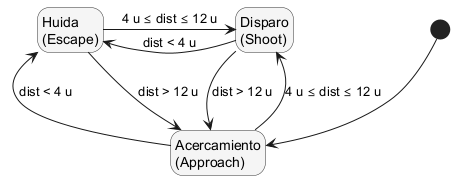
\includegraphics[width=0.95\textwidth,height=0.72\textheight,keepaspectratio]{Figuras/fsm_slimegreen.png}
\caption{
Diagrama de la FSM del SlimeGreen. \textit{Elaboración propia.}
}
\label{fig:placeholder-8}
\end{center}
\end{figure}


La implementación concreta en el método \texttt{Update()} del \texttt{SlimeGreen} muestra cómo la evaluación de distancia en cada fotograma sustituye a una tabla de transiciones explícita:

\begin{lstlisting}
protected override void Update() {
    base.Update();                                          // (1) Logica base: gracia, tiles
    
    if (isDead || player == null) return;                   // (2) Guardas de seguridad
    
    if (!IsAIEnabled) {                                     // (3) Periodo de gracia (0,75 s)
        StopMoving();
        return;
    }
    
    float distanceToPlayer = Vector2.Distance(              // (4) Distancia euclidiana
        transform.position, player.position);
    
    if (distanceToPlayer < escapeDistance) {                 // (5) FSM: transicion a Huida
        Escape();
    } else if (distanceToPlayer > maxDistance) {             // (6) FSM: transicion a Acercamiento
        Approach();
    } else {                                                // (7) FSM: estado Disparo
        StopMoving();
        if (Time.time >= nextShootTime) {
            Shoot();
        }
    }
    
    UpdateFallbackAnimation();                              // (8) Animacion procedural de respaldo
}
\end{lstlisting}


Línea por línea:

\begin{itemize}
\item \textbf{(1)} \texttt{base.Update()}: invoca el \texttt{Update()} de la clase base \texttt{Enemy}, que gestiona la interacción con tiles de velocidad y la detección de daño por contacto. Esta llamada es obligatoria en cualquier subclase que sobrescriba \texttt{Update()}, ya que sin ella los periodos de gracia y los modificadores de velocidad por tile dejarían de funcionar -- un ejemplo concreto de cómo el patrón \textit{Template Method} impone un contrato entre la clase base y las subclases.
\item \textbf{(2)} Las guardas \texttt{isDead} y \texttt{player == null} previenen la ejecución de lógica de IA sobre enemigos ya eliminados o cuando la referencia al jugador se ha perdido (por ejemplo, durante la transición de sala).
\item \textbf{(3)} \texttt{IsAIEnabled} es una propiedad de la clase base \texttt{Enemy} que compara \texttt{Time.time} con \texttt{aiEnabledTime}. Durante los primeros 0,75 segundos tras la aparición, esta propiedad devuelve \texttt{false}, y el enemigo permanece inactivo: esta ventana impide que el enemigo dispare al jugador en el mismo fotograma en que aparece.
\item \textbf{(4)} \texttt{Vector2.Distance} calcula la distancia euclidiana $d = \sqrt{(x_2 - x_1)^2 + (y_2 - y_1)^2}$ entre el enemigo y el jugador. Esta métrica se evalúa en cada fotograma (~60 veces por segundo con VSync activado), lo que produce transiciones de estado inmediatas cuando el jugador cruza un umbral de distancia.
\item \textbf{(5-7)} Las tres ramas del condicional implementan las transiciones de la FSM. La prioridad de evaluación es relevante: la condición de huida se evalúa \textit{antes} que la de disparo, garantizando que la autopreservación tiene prioridad sobre el ataque cuando el jugador está muy cerca.
\item \textbf{(8)} \texttt{UpdateFallbackAnimation()}: aplica una animación procedural de respaldo (oscilación de escala al moverse, pulso al disparar) cuando el \texttt{Animator} no dispone de un \texttt{AnimatorController} asignado. Esto garantiza retroalimentación visual incluso en configuraciones incompletas.
\end{itemize}

El comportamiento resultante es el de un enemigo que busca mantener una distancia óptima respecto al jugador: si este se acerca demasiado, el slime verde retrocede; si se aleja demasiado, el slime verde se aproxima; cuando se encuentra a la distancia ideal, se detiene y dispara proyectiles con una cadencia configurable.

\textbf{Análisis de la complejidad computacional de la FSM.} La evaluación de la FSM tiene coste $O(1)$ por fotograma: una llamada a \texttt{Vector2.Distance} (una raíz cuadrada) y tres comparaciones. Para los tres tipos de enemigo simultáneamente y una oleada típica de 8-12 enemigos, el coste total por fotograma es $O(n)$ donde $n$ es el número de enemigos activos -- despreciable frente al coste del renderizado y la simulación física.

\textbf{Sistema de disparo.} El método de disparo instancia un proyectil, le asigna una dirección calculada hacia la posición actual del jugador y le aplica una velocidad configurable. A continuación se muestra el código completo con comentarios exhaustivos:

\begin{lstlisting}
private void Shoot() {
    // Verificacion defensiva: si no hay prefab asignado, registrar advertencia
    if (projectilePrefab == null) {
        Debug.LogWarning("[SlimeGreen] No hay projectilePrefab asignado!");
        return;
    }
    
    // Calcular direccion normalizada desde el punto de disparo hacia el jugador.
    Vector2 direction = (player.position - shootPoint.position).normalized;
    
    // Instanciar proyectil en la posicion del punto de disparo,
    // sin rotacion (Quaternion.identity): la rotacion se aplica por velocidad.
    GameObject projectile = Instantiate(
        projectilePrefab, shootPoint.position, Quaternion.identity);
    
    // Aplicar multiplicadores de escala: escala de ajuste fino (20 % por defecto)
    // combinada con la escala de boss (> 1.0 para jefes).
    float finalScaleMultiplier = projectileScaleMultiplier * bossProjectileScale;
    projectile.transform.localScale *= finalScaleMultiplier;
    
    // Asignar velocidad al Rigidbody2D del proyectil.
    // Se garantiza una velocidad minima segura y se aplica el multiplicador (+15 %).
    Rigidbody2D projRb = projectile.GetComponent<Rigidbody2D>();
    float safeBaseSpeed = Mathf.Max(projectileSpeed, minProjectileBaseSpeed);
    float finalProjectileSpeed = safeBaseSpeed * projectileSpeedMultiplier;
    if (projRb != null) {
        projRb.linearVelocity = direction * finalProjectileSpeed;
    }
    
    // Asignar dano y escala externa al componente EnemyProjectile.
    EnemyProjectile projScript = projectile.GetComponent<EnemyProjectile>();
    if (projScript != null) {
        projScript.damage = projectileDamage;
        projScript.externalScaleMultiplier = finalScaleMultiplier;
    }
    
    // Actualizar la direccion del animator y activar animacion de disparo.
    SetAnimatorDirection(direction);
    TriggerShootAnimation();
    
    // Programar el siguiente disparo: Time.time + cooldown.
    nextShootTime = Time.time + shootCooldown;
}
\end{lstlisting}


\textbf{Mecánica de rebote contra muros.} Un aspecto diferenciador del SlimeGreen es su comportamiento al colisionar con los muros perimetrales durante el estado de huida. En lugar de quedarse atascado contra el muro -- lo que lo haría trivial de eliminar --, el enemigo calcula una nueva dirección de escape mediante reflexión vectorial:

\begin{lstlisting}
private void BounceFromWall(Collision2D collision) {
    if (collision.contactCount == 0) return;
    
    // Dirección deseada: alejarse del jugador
    Vector2 awayFromPlayer = (transform.position - player.position).normalized;
    // Normal de la superficie del muro en el punto de contacto
    Vector2 normal = collision.GetContact(0).normal;
    
    // Reflexión: dirección de movimiento reflejada respecto a la normal del muro
    Vector2 reflected = Vector2.Reflect(lastMoveDirection, normal).normalized;
    
    // Candidata: promedio entre la dirección de escape y la reflexión.
    Vector2 candidate = (awayFromPlayer + reflected).normalized;
    
    // Protección contra vector nulo: si el promedio se anula,
    // usar la reflexión pura o la dirección de escape como respaldo.
    if (candidate.sqrMagnitude < 0.0001f) {
        candidate = reflected.sqrMagnitude > 0.0001f ? reflected : awayFromPlayer;
    }
    
    // Corrección iterativa: si la candidata apunta hacia el jugador,
    // probar la tangente al muro como alternativa.
    for (int i = 0; i < wallBounceAttempts; i++) {
        Vector2 toPlayer = (player.position - transform.position).normalized;
        if (Vector2.Dot(candidate, toPlayer) < 0f) break;  // Ya se aleja: aceptar
        
        candidate = new Vector2(-normal.y, normal.x).normalized;
        if (Vector2.Dot(candidate, awayFromPlayer) < 0f) candidate = -candidate;
    }
    
    // Aplicar la nueva direccion
    lastMoveDirection = candidate;
    if (rb != null) {
        rb.linearVelocity = lastMoveDirection * lastAppliedMoveSpeed;
    }
}
\end{lstlisting}


Este algoritmo de rebote utiliza la fórmula de reflexión vectorial $\vec{r} = \vec{d} - 2(\vec{d} \cdot \vec{n})\vec{n}$, donde $\vec{d}$ es la dirección de movimiento y $\vec{n}$ es la normal de la superficie. La corrección iterativa garantiza que el enemigo no se dirija hacia el jugador tras el rebote, preservando la coherencia del comportamiento de huida.

\textbf{Limitador de velocidad.} Para evitar que ningun enemigo pueda ser mas rapido que el jugador -- lo que haria imposible la evasion --, se implementa un limitador de velocidad:

\begin{lstlisting}
private float CapToPlayerSpeed(float desiredSpeed) {
    if (playerController != null) {
        float playerSpeed = playerController.CurrentSpeed;
        if (playerSpeed > 0f)
            return Mathf.Min(desiredSpeed, playerSpeed);
    }
    return desiredSpeed;
}
\end{lstlisting}


\subsection{SlimeRed: enemigo perseguidor}


El \texttt{SlimeRed} implementa el comportamiento más directo de los tres tipos de enemigo. Su única estrategia consiste en calcular la dirección hacia el jugador y aplicar una velocidad constante en esa dirección:

\begin{lstlisting}
private void ChasePlayer() {
    Vector2 direction = (player.position - transform.position).normalized;
    
    if (rb != null) {
        rb.linearVelocity = direction * (moveSpeed * TileSpeedMultiplier);
    } else {
        transform.position = Vector2.MoveTowards(
            transform.position, 
            player.position, 
            (moveSpeed * TileSpeedMultiplier) * Time.deltaTime
        );
    }
    
    SetAnimatorAttacking(false);
}
\end{lstlisting}


El código contempla dos modos de movimiento: mediante \texttt{Rigidbody2D} (preferido, ya que respeta las colisiones físicas) y mediante \texttt{MoveTowards} (como respaldo en caso de que el componente de física no esté disponible). El multiplicador \texttt{TileSpeedMultiplier}, heredado de la clase base \texttt{Enemy}, permite que el efecto de los tiles de velocidad se aplique correctamente. La llamada a \texttt{SetAnimatorAttacking(false)} --método de la clase base que verifica la existencia del parámetro \texttt{IsAttacking} en el animator-- indica que el enemigo está persiguiendo y no atacando, lo que permite al animator reproducir la animación de movimiento correspondiente.

\subsection{SlimeBlue: enemigo saltador}


El \texttt{SlimeBlue} implementa un comportamiento basado en saltos rápidos (desplazamientos rápidos, \textit{dash}). A diferencia del SlimeGreen, cuya FSM tiene tres estados, el SlimeBlue implementa una \textbf{FSM de dos estados} con una separación clara entre la fase de espera y la fase de desplazamiento:

\begin{table}[H]
\begin{center}
\small
\begin{tabular}{|p{0.23\textwidth}|p{0.23\textwidth}|p{0.23\textwidth}|p{0.23\textwidth}|}
\hline
\textbf{Estado} & \textbf{Condición de entrada} & \textbf{Duración} & \textbf{Acción} \\ \hline
\textbf{Espera} (\textit{Idle}) & \texttt{isDashing == false} & Indefinida (hasta que se cumplan condiciones) & Enemigo estático (\texttt{rb.linearVelocity = Vector2.zero}); evalúa distancia al jugador y \textit{cooldown} \\ \hline
\textbf{Salto} (\textit{Dash}) & \texttt{minDashDistance <= dist <= maxDashDistance} AND \texttt{Time.time >= lastDashTime + dashCooldown} & Exactamente 0,4 s (\texttt{dashDuration}) & Desplazamiento rectilíneo a 12 u/s en dirección fija \\ \hline
\end{tabular}
\end{center}
\end{table}


\TablaTitulo{Estados y transiciones de la FSM del SlimeBlue.
}

\begin{figure}[H]
\begin{center}
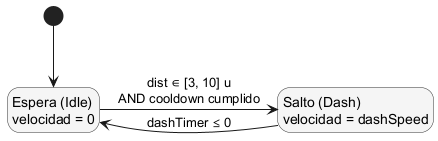
\includegraphics[width=0.95\textwidth,height=0.72\textheight,keepaspectratio]{Figuras/fsm_slimeblue.png}
\caption{
Diagrama de la FSM del SlimeBlue. \textit{Elaboración propia.}
}
\label{fig:placeholder-9}
\end{center}
\end{figure}


El método \texttt{Update()} del SlimeBlue implementa esta FSM de forma explícita, separando claramente las dos ramas de ejecución:

\begin{lstlisting}
protected override void Update() {
    base.Update();                                          // (1) Logica base heredada
    
    if (isDead || player == null) return;                   // (2) Guardas de seguridad
    
    if (!IsAIEnabled) {                                     // (3) Gracia: 0,75 s sin IA
        if (rb != null) rb.linearVelocity = Vector2.zero;
        return;
    }
    
    if (isDashing) {                                        // (4) Estado SALTO
        SetAnimatorDirection(dashDirection);                 //     Orientar animacion
        ApplyDashFacing();                                  //     Voltear todos los sprites
        dashTimer -= Time.deltaTime;                        //     Decrementar temporizador
        if (dashTimer <= 0f) {
            EndDash();                                      //     Transicion: Salto -> Espera
        }
    } else {                                                // (5) Estado ESPERA
        float distanceToPlayer = Vector2.Distance(
            transform.position, player.position);
        
        if (distanceToPlayer >= minDashDistance &&           // (6) Condicion de transicion
            distanceToPlayer <= maxDashDistance &&
            Time.time >= lastDashTime + dashCooldown) {
            StartDash();                                    //     Transicion: Espera -> Salto
        }
    }
    
    FlipSprite();                                           // (7) Orientacion visual
}
\end{lstlisting}


Línea por línea:

\begin{itemize}
\item \textbf{(1)} \texttt{base.Update()}: obligatorio para heredar la gestión de gracia y tiles de la clase base \texttt{Enemy} (patrón \textit{Template Method}).
\item \textbf{(4)} En el estado \textbf{Salto}, se actualizan la dirección del animator (\texttt{SetAnimatorDirection}) y el volteo de todos los \texttt{SpriteRenderer} del enemigo (\texttt{ApplyDashFacing}) en cada fotograma para reflejar la orientación del salto. El temporizador \texttt{dashTimer} se decrementa en cada fotograma. Cuando alcanza cero, se invoca \texttt{EndDash()}, que transita al estado \textbf{Espera} poniendo \texttt{isDashing = false}, deteniendo la velocidad y desactivando el flag de ataque del animator (\texttt{SetAnimatorAttacking(false)}).
\item \textbf{(5-6)} En el estado \textbf{Espera}, se evalúan tres condiciones conjuntas: distancia mínima (3 u), distancia máxima (10 u) y \textit{cooldown} cumplido (2 s desde el último salto). Las tres deben cumplirse simultáneamente para iniciar un nuevo salto.
\end{itemize}

La aplicación de velocidad se realiza en \texttt{FixedUpdate()}, separada de la lógica de decisión en \texttt{Update()}:

\begin{lstlisting}
private void FixedUpdate() {
    if (isDashing) {
        rb.linearVelocity = dashDirection * (dashSpeed * TileSpeedMultiplier);
    } else if (!isDead) {
        rb.linearVelocity = Vector2.zero;                   // Estatico entre saltos
    }
}
\end{lstlisting}


La separación \texttt{Update()} / \texttt{FixedUpdate()} es una decisión arquitectónica deliberada. La lógica de decisión de la FSM (¿debo saltar?) se ejecuta en \texttt{Update()} porque depende de la entrada del sistema y de temporizadores. La aplicación de velocidad al \texttt{Rigidbody2D} se ejecuta en \texttt{FixedUpdate()} porque el motor de física de Unity opera a frecuencia fija (50 Hz por defecto), y aplicar velocidad en \texttt{Update()} produciría movimiento inconsistente a distintas tasas de fotogramas.

La dirección del salto se calcula en el momento de su inicio (\texttt{StartDash()}) y permanece fija durante toda la duración del desplazamiento. Esto permite al jugador anticipar la trayectoria del salto y esquivarlo, introduciendo una componente táctica en el enfrentamiento contra este tipo de enemigo. Los parámetros del salto son: velocidad de doce unidades por segundo, duración de 0,4 segundos y tiempo de espera de dos segundos entre saltos consecutivos.

\begin{figure}[H]
\begin{center}
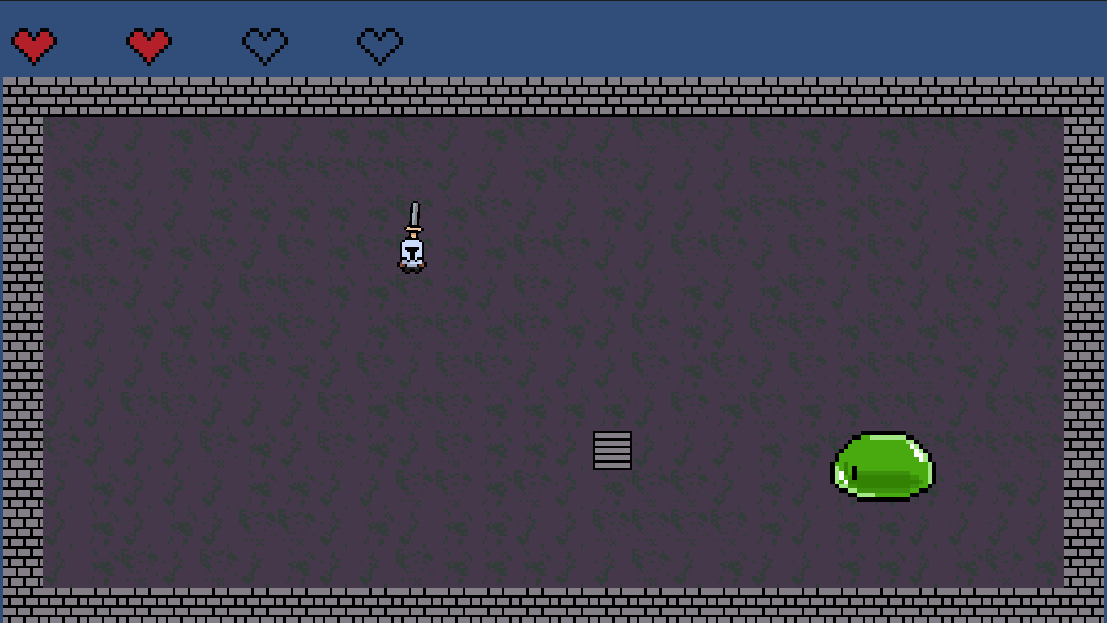
\includegraphics[width=0.9\textwidth]{Figuras/Jefe.png}
\caption{Captura de pantalla de \textit{Ascension} durante un encuentro con un enemigo jefe, mostrando el incremento visual de tamaño respecto a los enemigos estándar y los proyectiles de mayor escala. \textit{Elaboración propia.}}
\label{fig:placeholder-10}
\end{center}
\end{figure}


\textbf{Visualización durante el desarrollo.} Se implementan \textit{Gizmos} para facilitar el ajuste del rango de salto:

\begin{lstlisting}
private void OnDrawGizmosSelected() {
    Gizmos.color = Color.yellow;
    Gizmos.DrawWireSphere(transform.position, minDashDistance);
    
    Gizmos.color = Color.cyan;
    Gizmos.DrawWireSphere(transform.position, maxDashDistance);
}
\end{lstlisting}

\subsection{EnemyManager: gestión de aparición de enemigos}


El \texttt{EnemyManager} es responsable de la instanciación de enemigos en cada sala, la gestión de referencias a los enemigos activos y la detección de sala completada. Soporta dos modos de aparición:

\textbf{Modo por presupuesto de coste.} El sistema dispone de un presupuesto numérico y selecciona enemigos aleatoriamente -- ponderados por peso -- hasta agotar el presupuesto. Este mecanismo implementa una curva de dificultad \textbf{emergente}: a medida que el presupuesto crece con la profundidad de la mazmorra, el sistema puede instanciar combinaciones más peligrosas (por ejemplo, dos slimes verdes y tres rojos en lugar de solo cuatro rojos), sin necesidad de tablas de dificultad codificadas manualmente.

\begin{lstlisting}
public void SpawnByCost(Rect area, int maxCost, int depth) {
    int remaining = maxCost;                                 // (1) Presupuesto disponible
    int safety = 200;
    int spawned = 0;
    
    while (remaining >= minCost && safety-- > 0) {           // (2) Bucle de aparicion
        int totalWeight = 0;                                 // (3) Seleccion ponderada
        foreach (var a in available)
            if (a.cost <= remaining) totalWeight += a.weight;
        if (totalWeight == 0) break;
        
        int roll = Random.Range(0, totalWeight);
        GameObject chosen = null; int chosenCost = 0;
        foreach (var a in available) {
            if (a.cost > remaining) continue;
            roll -= a.weight;
            if (roll < 0) { chosen = a.prefab; chosenCost = a.cost; break; }
        }
        if (chosen == null) break;
        
        Vector2 pos = GetSafeSpawnPosition(area);            // (4) Posicion segura
        var instance = Instantiate(chosen, pos,              // (5) Instanciacion
                                   Quaternion.identity);
        
        remaining -= chosenCost;                             // (6) Decrementar presupuesto
        spawned++;
    }
}
\end{lstlisting}


Línea por línea:

\begin{itemize}
\item \textbf{(1)} \texttt{remaining} representa el presupuesto disponible para la sala actual. El presupuesto base se incrementa con \texttt{depth} (profundidad de la mazmorra), produciendo oleadas progresivamente más intensas.
\item \textbf{(2)} El bucle continúa mientras quede presupuesto suficiente para al menos el enemigo más barato (\texttt{minCost}). La variable \texttt{safety} previene bucles infinitos en caso de error de configuración (por ejemplo, si todos los costes de enemigos exceden el presupuesto restante).
\item \textbf{(3)} La selección ponderada recorre la lista de enemigos cuyo coste no exceda el presupuesto restante, acumulando sus pesos. Un valor aleatorio (\texttt{roll}) determina cuál se selecciona, de modo que enemigos con mayor peso aparecen con mayor frecuencia: un slime rojo (peso alto, coste bajo) aparece más a menudo que un slime verde (peso medio, coste alto), reflejando la intención de diseño de que el enemigo francotirador sea menos común.
\item \textbf{(4-5)} El posicionamiento seguro garantiza que ningún enemigo aparezca sobre el jugador.
\item \textbf{(6)} Decrementar el presupuesto tras instanciar produce un reparto orgánico: con presupuesto alto, el sistema puede «gastar» en enemigos caros o repartir en muchos baratos, produciendo composiciones de oleada variadas en cada sala.
\end{itemize}

\textbf{Posicionamiento seguro.} La función \texttt{GetSafeSpawnPosition} evita que los enemigos aparezcan demasiado cerca del jugador, realizando hasta 25 intentos de posicionamiento aleatorio antes de recurrir a una posición de respaldo:

\begin{lstlisting}
private Vector2 GetSafeSpawnPosition(Rect area) {
    Vector2 fallback = new Vector2(
        Random.Range(area.xMin, area.xMax),
        Random.Range(area.yMin, area.yMax));
    
    var player = GameObject.FindGameObjectWithTag("Player");
    if (player == null) return fallback;
    
    Vector2 playerPos = player.transform.position;
    float minDistSqr = safeSpawnRadius * safeSpawnRadius;
    
    for (int i = 0; i < safeSpawnAttempts; i++) {
        Vector2 candidate = new Vector2(
            Random.Range(area.xMin, area.xMax),
            Random.Range(area.yMin, area.yMax));
        if ((candidate - playerPos).sqrMagnitude >= minDistSqr)
            return candidate;
    }
    
    return fallback;
}
\end{lstlisting}


\textbf{Detección de sala completada.} En cada fotograma, el gestor elimina las referencias a enemigos destruidos y evalúa si todos los enemigos han sido eliminados. Cuando esto ocurre, emite un evento que desencadena la habilitación de las escaleras de progresión:

\begin{lstlisting}
void Update() {
    if (!roomActive) return;
    
    PruneTracked();  // Eliminar referencias nulas
    
    if (trackedEnemies.Count == 0) {
        roomActive = false;
        roomCleared = true;
        
        if (!suppressClearEvent) {
            OnRoomCleared?.Invoke();
        }
    }
}
\end{lstlisting}


\subsection{Configuración de enemigos: EnemyData}


Los datos de cada tipo de enemigo se definen mediante \textit{ScriptableObjects}. Se seleccionó este mecanismo frente a la codificación de estadísticas en los propios scripts de enemigo por la misma razón expuesta para los datos de armas: durante el desarrollo, los parámetros de equilibrado de los enemigos (vida, daño, velocidad, coste de aparición) se ajustaron iterativamente más de diez veces, y cada ajuste con \textit{ScriptableObjects} es inmediato y no requiere recompilación.

\begin{lstlisting}
[CreateAssetMenu(menuName = "Enemies/EnemyData")]
public class EnemyData : ScriptableObject {
    public string enemyName;      // Identificador visible ("Slime Verde")
    public int maxHealth = 3;     // Puntos de vida maximos
    public int damage = 1;        // Dano infligido por contacto o proyectil
    public float speed = 2f;      // Velocidad base en unidades/segundo
    public Sprite sprite;         // Sprite principal del enemigo
    public int enemyCost;         // Coste de aparicion en el sistema de presupuesto
}
\end{lstlisting}


El campo \texttt{enemyCost} merece una explicación específica: define cuánto "cuesta" instanciar este enemigo dentro del sistema de presupuesto del \texttt{EnemyManager}. Un slime rojo (perseguidor, fácil de esquivar) tiene un coste bajo, mientras que un slime verde (francotirador, más peligroso) tiene un coste superior. El presupuesto total del \texttt{EnemyManager} se incrementa con la profundidad de la mazmorra, produciendo oleadas progresivamente más intensas sin necesidad de tablas de dificultad codificadas manualmente. Esta decisión reduce el acoplamiento entre el sistema de dificultad y los tipos de enemigo: añadir un nuevo tipo de enemigo con su \texttt{enemyCost} correspondiente integra automáticamente ese enemigo en la curva de dificultad sin modificar el código del \texttt{EnemyManager}.

\subsection{Síntesis comparativa de los tipos de enemigo}


La siguiente tabla resume las diferencias de comportamiento, parámetros y rol táctico entre los tres tipos de enemigo, mostrando cómo la jerarquía basada en el patrón \textit{Template Method} permite diferenciar la IA sin duplicar la lógica base compartida:

\begin{table}[H]
\begin{center}
\small
\begin{tabular}{|p{0.23\textwidth}|p{0.23\textwidth}|p{0.23\textwidth}|p{0.23\textwidth}|}
\hline
\textbf{Aspecto} & \textbf{SlimeRed (perseguidor)} & \textbf{SlimeGreen (francotirador)} & \textbf{SlimeBlue (saltador)} \\ \hline
Comportamiento de IA & Persecución directa constante & FSM de 3 estados (huir, acercarse, disparar) & Ciclo de espera y salto (\textit{dash}) \\ \hline
Método principal sobrescrito & \texttt{Update()} -> \texttt{ChasePlayer()} & \texttt{Update()} -> \texttt{Escape()} / \texttt{Approach()} / \texttt{Shoot()} & \texttt{Update()} -> \texttt{StartDash()} / \texttt{EndDash()} \\ \hline
Movimiento & \texttt{rb.linearVelocity} hacia el jugador & \texttt{rb.linearVelocity} según zona de distancia & \texttt{rb.linearVelocity} solo durante el salto \\ \hline
Distancia al jugador & Siempre se acerca (0 m ideales) & Mantiene distancia óptima (4–12 unidades) & Rango de activación (3–10 unidades) \\ \hline
Mecánica de daño & Contacto directo & Proyectil a distancia (\texttt{EnemyProjectile}) & Contacto durante el salto \\ \hline
Velocidad base & \texttt{moveSpeed} $\times$ \texttt{TileSpeedMultiplier} & Limitada por \texttt{CapToPlayerSpeed} & \texttt{dashSpeed} = 12 u/s durante 0,4 s \\ \hline
Tiempo de espera & Ninguno (acción continua) & \texttt{shootCooldown} entre disparos & \texttt{dashCooldown} = 2 s entre saltos \\ \hline
Coste de aparición & Bajo (fácil de esquivar) & Alto (peligroso a distancia) & Medio (predecible pero rápido) \\ \hline
Rol táctico & Presión constante, obliga a moverse & Obliga a cerrar distancia o usar arma a distancia & Requiere anticipación y esquiva \\ \hline
Contramedida del jugador & Arma cuerpo a cuerpo y kiting & Arma a distancia o persecución rápida & Esquiva (\textit{roll}) y posicionamiento \\ \hline
\end{tabular}
\end{center}
\end{table}


\TablaTitulo{Comparativa de comportamiento, parámetros y rol táctico de los tres tipos de enemigo.
}

La diversidad de estos tres arquetipos, combinada con el sistema de presupuesto de coste del \texttt{EnemyManager} y la variabilidad de los tiles especiales, produce situaciones de combate tácticas y diferenciadas en cada sala sin necesidad de un repertorio extenso de tipos de enemigo.

\subsection{Diagrama de flujo de decisión de la IA por tipo de enemigo}


El siguiente diagrama de flujo unificado muestra la lógica de decisión completa que ejecuta cada tipo de enemigo en cada fotograma, incluyendo la lógica heredada de la clase base \texttt{Enemy} (común a los tres) y la lógica específica de cada subclase:

\begin{figure}[H]
\begin{center}
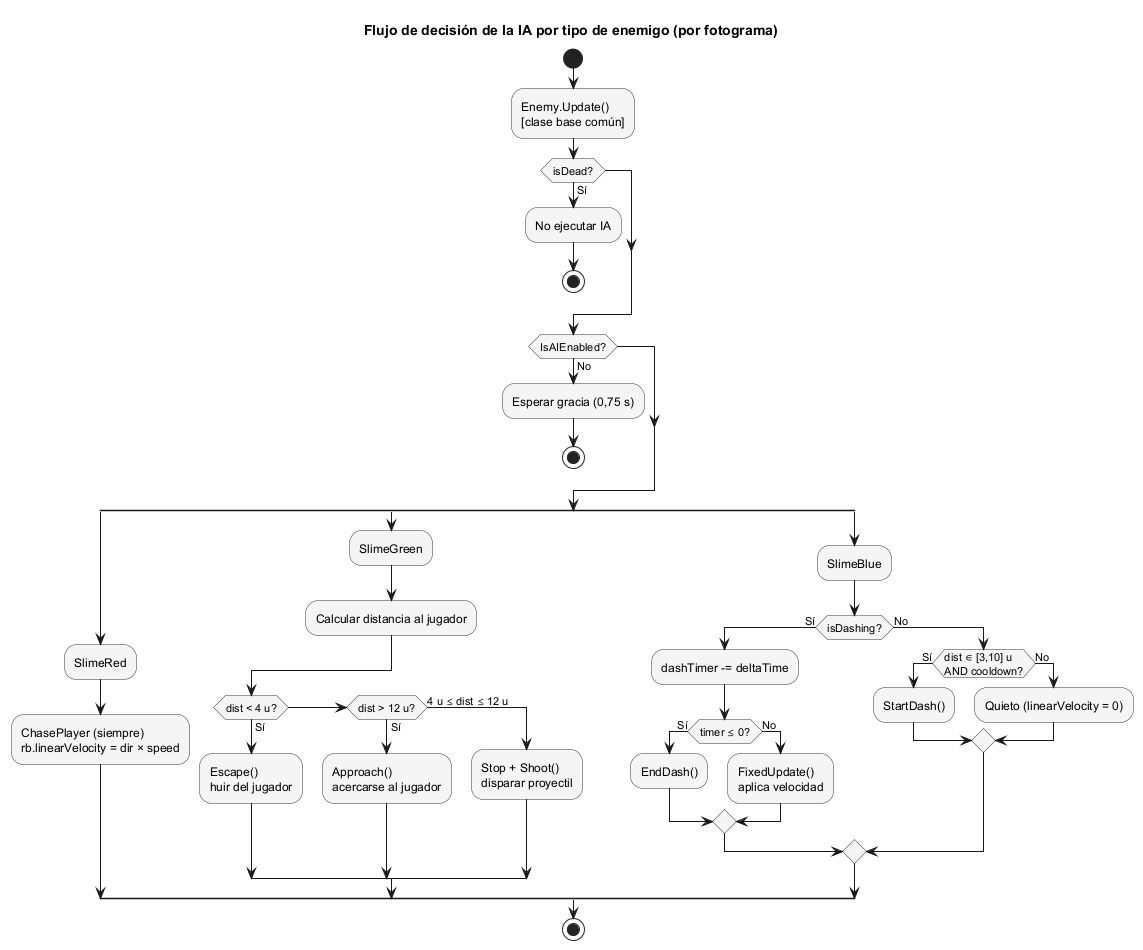
\includegraphics[width=0.95\textwidth,height=0.72\textheight,keepaspectratio]{Figuras/flujo_decision_ia.png}
\caption{
Diagrama de flujo de decisión de la IA por tipo de enemigo. \textit{Elaboración propia.}
}
\label{fig:placeholder-12}
\end{center}
\end{figure}


Este diagrama evidencia una propiedad del diseño: la lógica heredada de la clase base \texttt{Enemy} (verificaciones de muerte, gracia y tiles) se ejecuta siempre \textit{antes} que la lógica específica de cada subclase, garantizando que las comprobaciones de seguridad son comunes e inmutables --un ejemplo concreto del contrato impuesto por el patrón \textit{Template Method}.

\begin{figure}[H]
\begin{center}
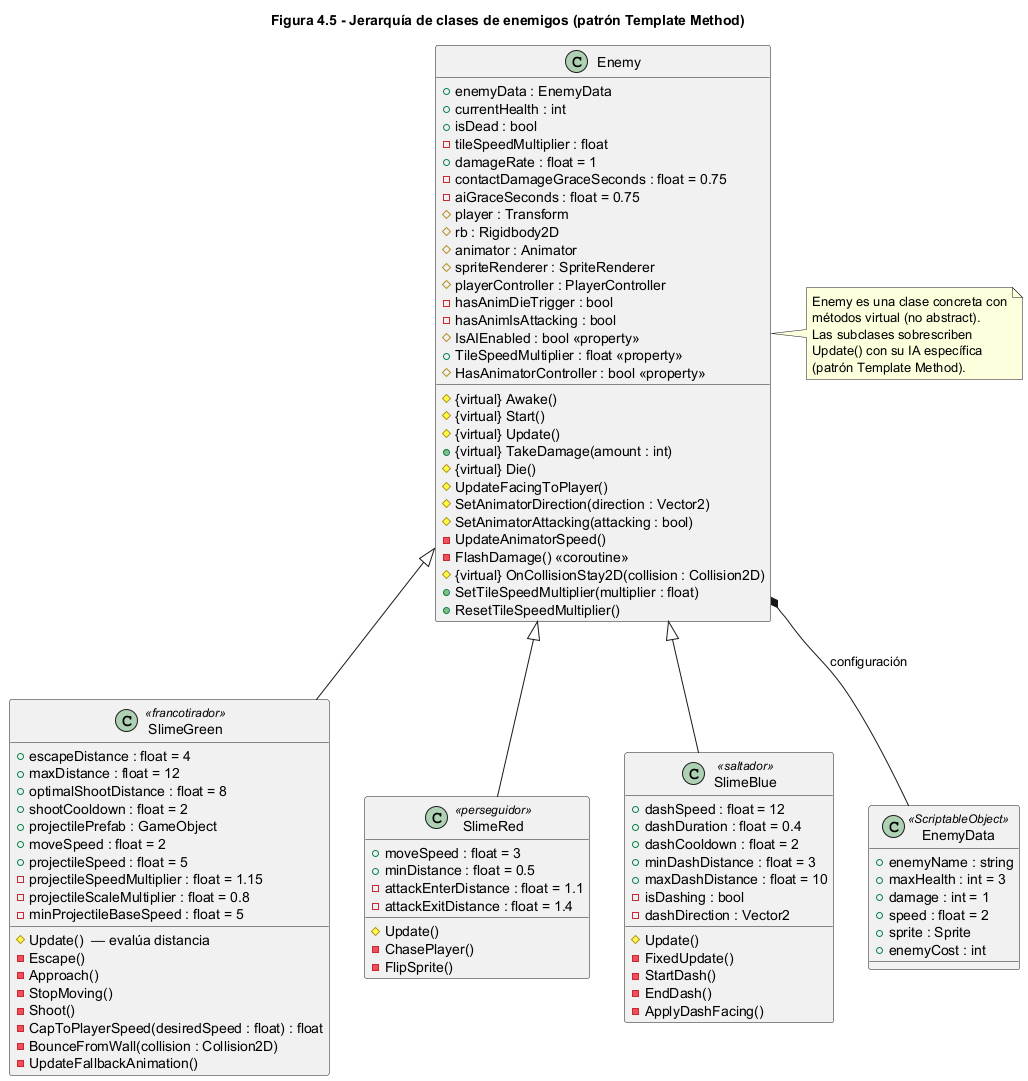
\includegraphics[width=0.95\textwidth,height=0.72\textheight,keepaspectratio]{Figuras/figura4_5_clases_enemigos.png}
\caption{
Diagrama de clases UML de la jerarquía de enemigos. \textit{Elaboración propia.}
}
\label{fig:placeholder-13}
\end{center}
\end{figure}


\begin{figure}[H]
\begin{center}
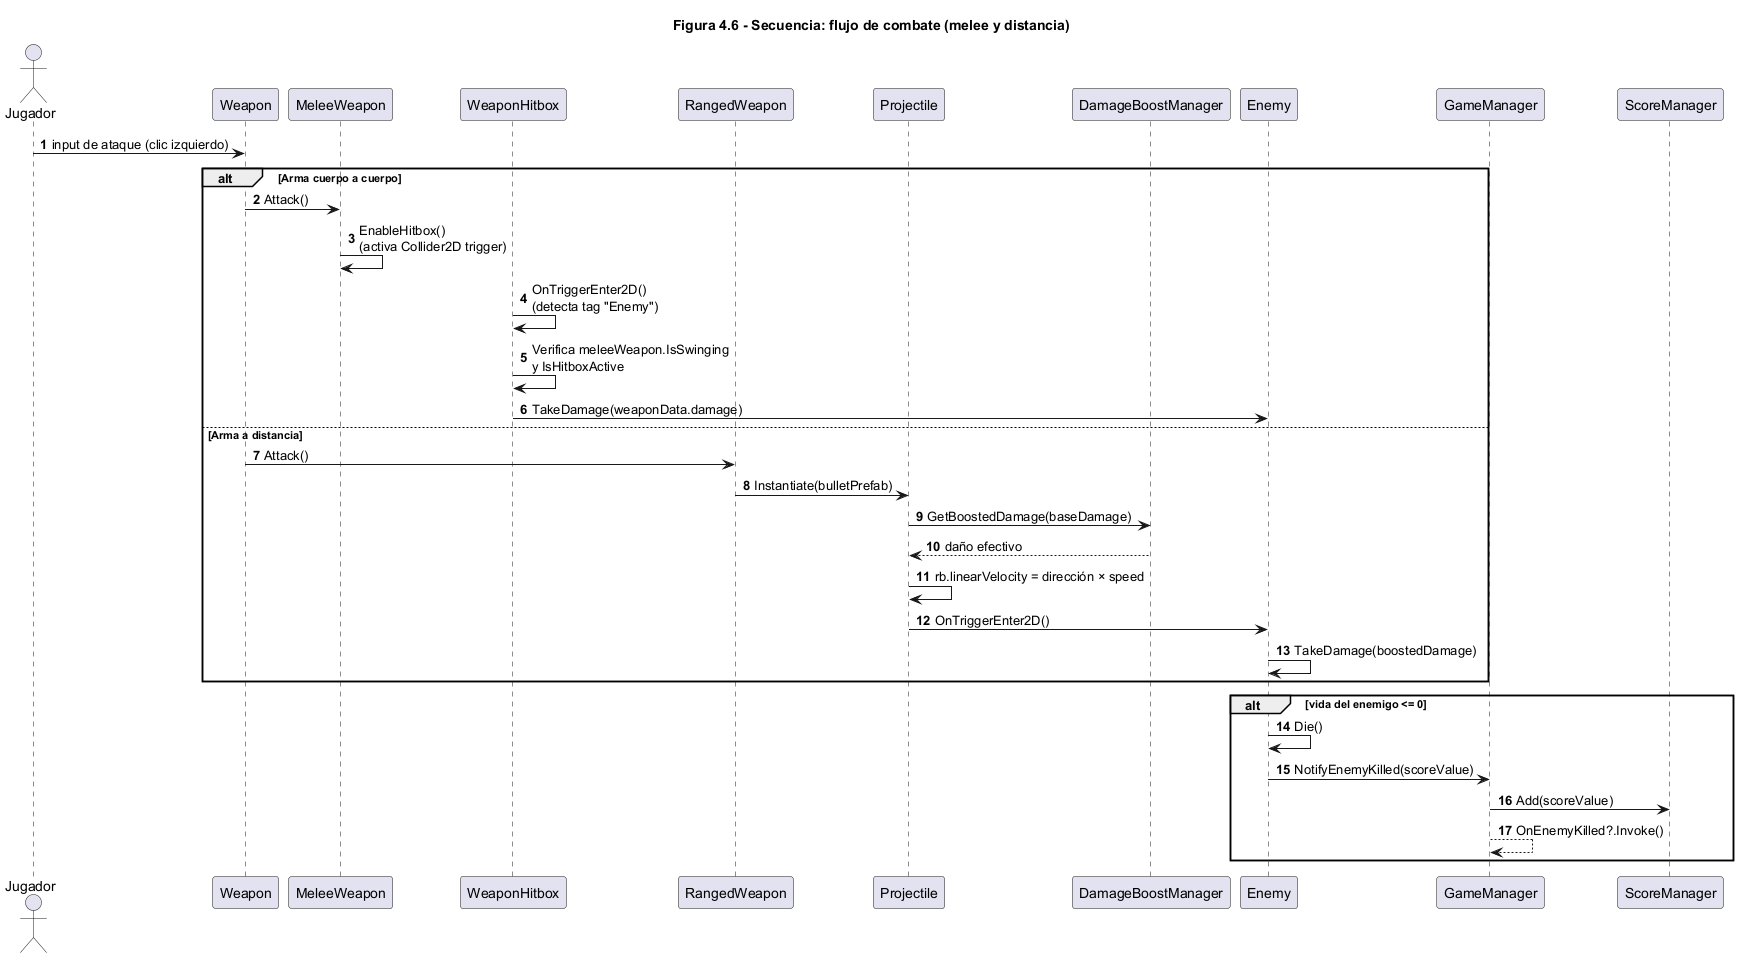
\includegraphics[width=0.95\textwidth,height=0.72\textheight,keepaspectratio]{Figuras/figura4_6_secuencia_combate.png}
\caption{
Diagrama de secuencia UML del flujo de combate. \textit{Elaboración propia.}
}
\label{fig:placeholder-14}
\end{center}
\end{figure}


\section{Sistema de armas y combate}


\textbf{Evolución iterativa.} El sistema de armas pasó por dos rediseños. La primera versión implementaba una clase única \texttt{Weapon} con un enumerado \texttt{WeaponType} y bloques condicionales que diferenciaban el comportamiento cuerpo a cuerpo del comportamiento a distancia; esta estructura se volvió difícil de mantener al añadir los efectos visuales (\textit{weapon trail}, parpadeo de hitbox), ya que cada tipo de arma requería campos y lógica distintos dentro de la misma clase. La refactorización al patrón \textit{Strategy} -- con \texttt{Weapon} como clase base y \texttt{MeleeWeapon} / \texttt{RangedWeapon} como estrategias concretas -- resolvió este problema. La animación de barrido del arma cuerpo a cuerpo se rediseñó de interpolación lineal a sinusoidal tras observar que el movimiento uniforme transmitía una sensación mecánica carente del «peso» visual esperado en un arma.

\subsection{Weapon: clase base del sistema de armas y patrón \textit{Strategy}}


El sistema de armas implementa el patrón \textit{Strategy}. Se seleccionó este patrón frente a la alternativa de una única clase \texttt{Weapon} con un enumerado \texttt{WeaponType} y bloques condicionales (\texttt{if (type == Melee) ... else if (type == Ranged) ...}). Esta alternativa se descartó por dos razones: en primer lugar, cada tipo de arma requiere campos específicos distintos -- \texttt{swingAngle} y \texttt{swingDuration} para las armas cuerpo a cuerpo, \texttt{bulletPrefab} y \texttt{attackCooldown} para las armas a distancia --, lo que produciría una clase con campos que solo son relevantes para uno de los tipos; en segundo lugar, añadir un tercer tipo de arma obligaría a modificar la lógica interna de la clase existente, violando el principio de apertura-cierre.

El patrón \textit{Strategy} resuelve ambos problemas: la clase base \texttt{Weapon} define la interfaz común (\texttt{Attack()}, rotación hacia el cursor, órbita alrededor del jugador) y las subclases \texttt{MeleeWeapon} y \texttt{RangedWeapon} encapsulan únicamente los campos y la lógica relevantes para su tipo de ataque.

\textbf{Sistema de rotación y órbita.} El arma sigue la posición del cursor del ratón y orbita alrededor del jugador:

\begin{lstlisting}
private void RotateTowardsMouse() {
    Vector3 mouseWorldPosition = camera.ScreenToWorldPoint(Input.mousePosition);
    mouseWorldPosition.z = 0;
    
    Vector2 direction = (mouseWorldPosition - transform.position).normalized;
    float angle = Mathf.Atan2(direction.y, direction.x) * Mathf.Rad2Deg;
    
    float spriteOrientationOffset = -90f;
    transform.rotation = Quaternion.Euler(0, 0, angle + spriteOrientationOffset);
}
\end{lstlisting}


La conversión de la posición del ratón de coordenadas de pantalla a coordenadas del mundo se realiza mediante \texttt{Camera.ScreenToWorldPoint}. El ángulo de rotación se calcula mediante \texttt{Mathf.Atan2(direction.y, direction.x)}, que retorna el ángulo en radianes del vector dirección respecto al eje X positivo; la multiplicación por \texttt{Mathf.Rad2Deg} convierte a grados para aplicarlo como rotación del \texttt{transform}. El desplazamiento de -90º (\texttt{spriteOrientationOffset}) compensa que los sprites de las armas están orientados hacia arriba en su fichero de origen: sin este ajuste, un ángulo de 0º apuntaría el sprite hacia la derecha en lugar de hacia arriba.

Se seleccionó el cálculo trigonométrico (\texttt{Atan2} + rotación Euler) frente a la alternativa de usar \texttt{Quaternion.LookRotation}, porque esta última está orientada al espacio 3D y requiere una conversión adicional para obtener una rotación exclusivamente en el eje Z, lo que introduce complejidad innecesaria en un proyecto 2D.

\subsection{MeleeWeapon: armas cuerpo a cuerpo}


El \texttt{MeleeWeapon} implementa un ataque de barrido (\textit{swing}) con un arco configurable de 180 grados y una animación procedural:

\begin{lstlisting}
protected override void Update() {
    base.Update();
    
    // Cancelar swing si el jugador suelta el boton del raton a mitad de ataque
    if (!Input.GetMouseButton(0) && isSwinging) {
        StopSwinging();
        return;
    }
    
    if (isSwinging) {
        swingTimer += Time.deltaTime;
        float progress = swingTimer / swingDuration;
        
        if (progress >= 1f) {
            StopSwinging();
        } else {
            float smoothProgress = Mathf.Sin(progress * Mathf.PI);
            float currentSwingOffset = Mathf.Lerp(
                -swingAngle / 2, 
                swingAngle / 2, 
                smoothProgress
            );
            
            Vector3 currentRotation = transform.localEulerAngles;
            currentRotation.z = swingStartAngle + currentSwingOffset;
            transform.localRotation = Quaternion.Euler(currentRotation);
        }
    }
}
\end{lstlisting}


La animación del barrido utiliza una curva sinusoidal (\texttt{Mathf.Sin}) para producir un movimiento suave que acelera al inicio y desacelera al final, resultando en una sensación de peso y naturalidad. Se seleccionó la interpolación sinusoidal frente a una interpolación lineal (\texttt{Mathf.Lerp} con progreso lineal) porque esta última produce un movimiento uniforme que transmite una sensación mecánica, carente del «peso» visual que se espera de un arma cuerpo a cuerpo. Si el jugador suelta el botón del ratón durante el barrido, este se cancela inmediatamente mediante \texttt{StopSwinging()}, que centraliza la desactivación de la hitbox y el rastro visual (\texttt{WeaponTrail}) en un único método, evitando la duplicación de lógica de limpieza.

Línea por línea del fragmento:

\begin{itemize}
\item \texttt{swingTimer += Time.deltaTime}: acumula el tiempo transcurrido desde el inicio del barrido, independientemente de la tasa de fotogramas.
\item \texttt{float progress = swingTimer / swingDuration}: normaliza el progreso del barrido al rango [0, 1], donde 0 es el inicio y 1 es el final.
\item \texttt{Mathf.Sin(progress * Mathf.PI)}: convierte el progreso lineal en una curva sinusoidal. Cuando \texttt{progress = 0}, el seno vale 0; cuando \texttt{progress = 0.5}, vale 1 (máximo desplazamiento); cuando \texttt{progress = 1}, vuelve a 0.
\item \texttt{Mathf.Lerp(-swingAngle/2, swingAngle/2, smoothProgress)}: mapea el progreso sinusoidal a un ángulo de rotación dentro del rango [-90º, +90º], produciendo el arco de 180º configurable.
\item \texttt{StopSwinging()}: al completar el barrido (\texttt{progress >= 1}) o al soltar el botón, desactiva la hitbox, detiene el rastro visual y marca \texttt{isSwinging = false}.
\end{itemize}

\textbf{Detección de impacto.} Durante el barrido, la hitbox del arma detecta colisiones con enemigos. Si existen componentes \texttt{WeaponHitbox} hijos, la detección se delega a ellos para evitar daño duplicado; en caso contrario, el propio \texttt{MeleeWeapon} verifica las condiciones de activación:

\begin{lstlisting}
private void OnTriggerEnter2D(Collider2D other) {
    // Si hay WeaponHitbox hijos, ellos gestionan el dano
    if (weaponHitboxes != null && weaponHitboxes.Length > 0) return;
    if (!isSwinging || !hitboxesActive) return;
    if (hitbox == null || !hitbox.enabled) return;
    
    if (other.CompareTag("Enemy") && weaponData != null) {
        Enemy enemy = other.GetComponent<Enemy>();
        if (enemy != null)
            enemy.TakeDamage(weaponData.damage);
    }
}
\end{lstlisting}


\subsection{RangedWeapon: armas a distancia}


El \texttt{RangedWeapon} implementa el ataque mediante la instanciación de proyectiles:

\begin{lstlisting}
public override void Attack() {
    if (Time.time < lastAttackTime + attackCooldown) return;
    
    if (weaponData?.bulletPrefab != null) {
        lastAttackTime = Time.time;
        
        Vector3 spawnPosition = spawner?.position ?? transform.position;
        Quaternion spawnRotation = transform.rotation;
        
        GameObject bullet = Instantiate(
            weaponData.bulletPrefab, 
            spawnPosition, 
            spawnRotation
        );
        
        Projectile projectileScript = bullet.GetComponent<Projectile>();
        if (projectileScript != null) {
            projectileScript.damage = weaponData.damage;
            projectileScript.speed = 10f;
        }
    }
}
\end{lstlisting}


El operador \texttt{?.} (operador condicional nulo) evita excepciones cuando una referencia es nula. El operador \texttt{??} (operador de coalescencia nula) proporciona un valor de respaldo cuando el valor principal es nulo.

\subsection{Projectile: comportamiento de proyectiles}


El componente \texttt{Projectile} controla el movimiento lineal del proyectil, su autodestrucción por tiempo de vida y la integración con el sistema de bonificación de daño:

\begin{lstlisting}
void Start() {
    if (DamageBoostManager.Instance != null) {
        damage = DamageBoostManager.Instance.GetBoostedDamage(damage);
    }
    
    if (rb != null) {
        rb.linearVelocity = transform.up * speed;
    }
    
    Destroy(gameObject, lifetime);
}
\end{lstlisting}


La consulta al \texttt{DamageBoostManager} permite que los proyectiles se beneficien de las bonificaciones de daño otorgadas por los tiles de potenciación. La llamada a \texttt{Destroy(gameObject, lifetime)} programa la destrucción automática del proyectil tras un tiempo configurable, evitando la acumulación de objetos fuera de los límites de la sala.

\textbf{Detección de impacto.} Al colisionar, el proyectil aplica daño a los enemigos y se destruye al contactar con paredes o enemigos. Los proyectiles del jugador ignoran explícitamente las armas del propio jugador para evitar colisiones involuntarias:

\begin{lstlisting}
void OnTriggerEnter2D(Collider2D other) {
    if (other.CompareTag("Player") || other.CompareTag("Weapon")
        || other.GetComponent<Weapon>() != null)
        return;
    
    if (other.CompareTag("Enemy")) {
        Enemy enemy = other.GetComponent<Enemy>();
        if (enemy != null)
            enemy.TakeDamage(damage);
    }
    
    if (other.CompareTag("Wall") || other.CompareTag("Enemy"))
        Destroy(gameObject);
}
\end{lstlisting}


La comprobación combinada de la etiqueta \texttt{"Weapon"} y del componente \texttt{Weapon} proporciona una doble verificación: la etiqueta cubre los casos estándar, mientras que la comprobación de componente cubre prefabs que pudieran no tener la etiqueta asignada.

\subsection{WeaponData: configuración de armas mediante \textit{ScriptableObjects}}


Los datos de cada arma se definen mediante \textit{ScriptableObjects}, manteniendo la separación entre datos y lógica. Al igual que con \texttt{PlayerClass} y \texttt{EnemyData}, se seleccionó este mecanismo frente a la codificación directa de parámetros en los scripts de arma. Esta decisión permite que el mismo prefab de \texttt{MeleeWeapon} se reutilice con distintas configuraciones (espada, hacha, lanza) simplemente asignando un \textit{ScriptableObject} diferente, sin duplicar prefabs ni código:

\begin{lstlisting}
[CreateAssetMenu(menuName = "Items/WeaponData")]
public class WeaponData : ScriptableObject {
    public string weaponName;         // Nombre visible del arma
    public int damage;                // Dano base por impacto
    public float atackSpeed;          // Velocidad de ataque (tiempo de espera entre ataques)
    public Sprite sprite;             // Sprite visual del arma
    public GameObject bulletPrefab;   // Prefab del proyectil (solo para armas a distancia; null para melee)
    public GameObject weaponPrefab;   // Prefab del GameObject completo del arma
}
\end{lstlisting}


Línea por línea:

\begin{itemize}
\item \texttt{damage}: daño base que puede ser modificado en tiempo de ejecución por el \texttt{DamageBoostManager} cuando el jugador se encuentra sobre un tile de potenciación.
\item \texttt{bulletPrefab}: referencia condicional -- solo las armas a distancia la utilizan; las armas cuerpo a cuerpo la dejan como \texttt{null}. El código de \texttt{RangedWeapon.Attack()} verifica esta referencia antes de instanciar proyectiles mediante el operador condicional nulo (\texttt{?.}).
\item \texttt{weaponPrefab}: referencia al prefab preconfigurado que incluye el componente \texttt{MeleeWeapon} o \texttt{RangedWeapon}, los colisionadores, el \textit{SpriteRenderer} y los efectos visuales.
\end{itemize}

\subsection{Flujo completo de daño: del ataque a la puntuación}


El sistema de combate involucra a cinco componentes distribuidos en tres subsistemas (armas, enemigos y gestión central). El siguiente diagrama describe la cadena completa de invocaciones que se produce cuando el jugador ataca a un enemigo, desde la entrada del jugador hasta la actualización de la puntuación:
\vspace{-0.5em}
\begin{figure}[H]
\begin{center}
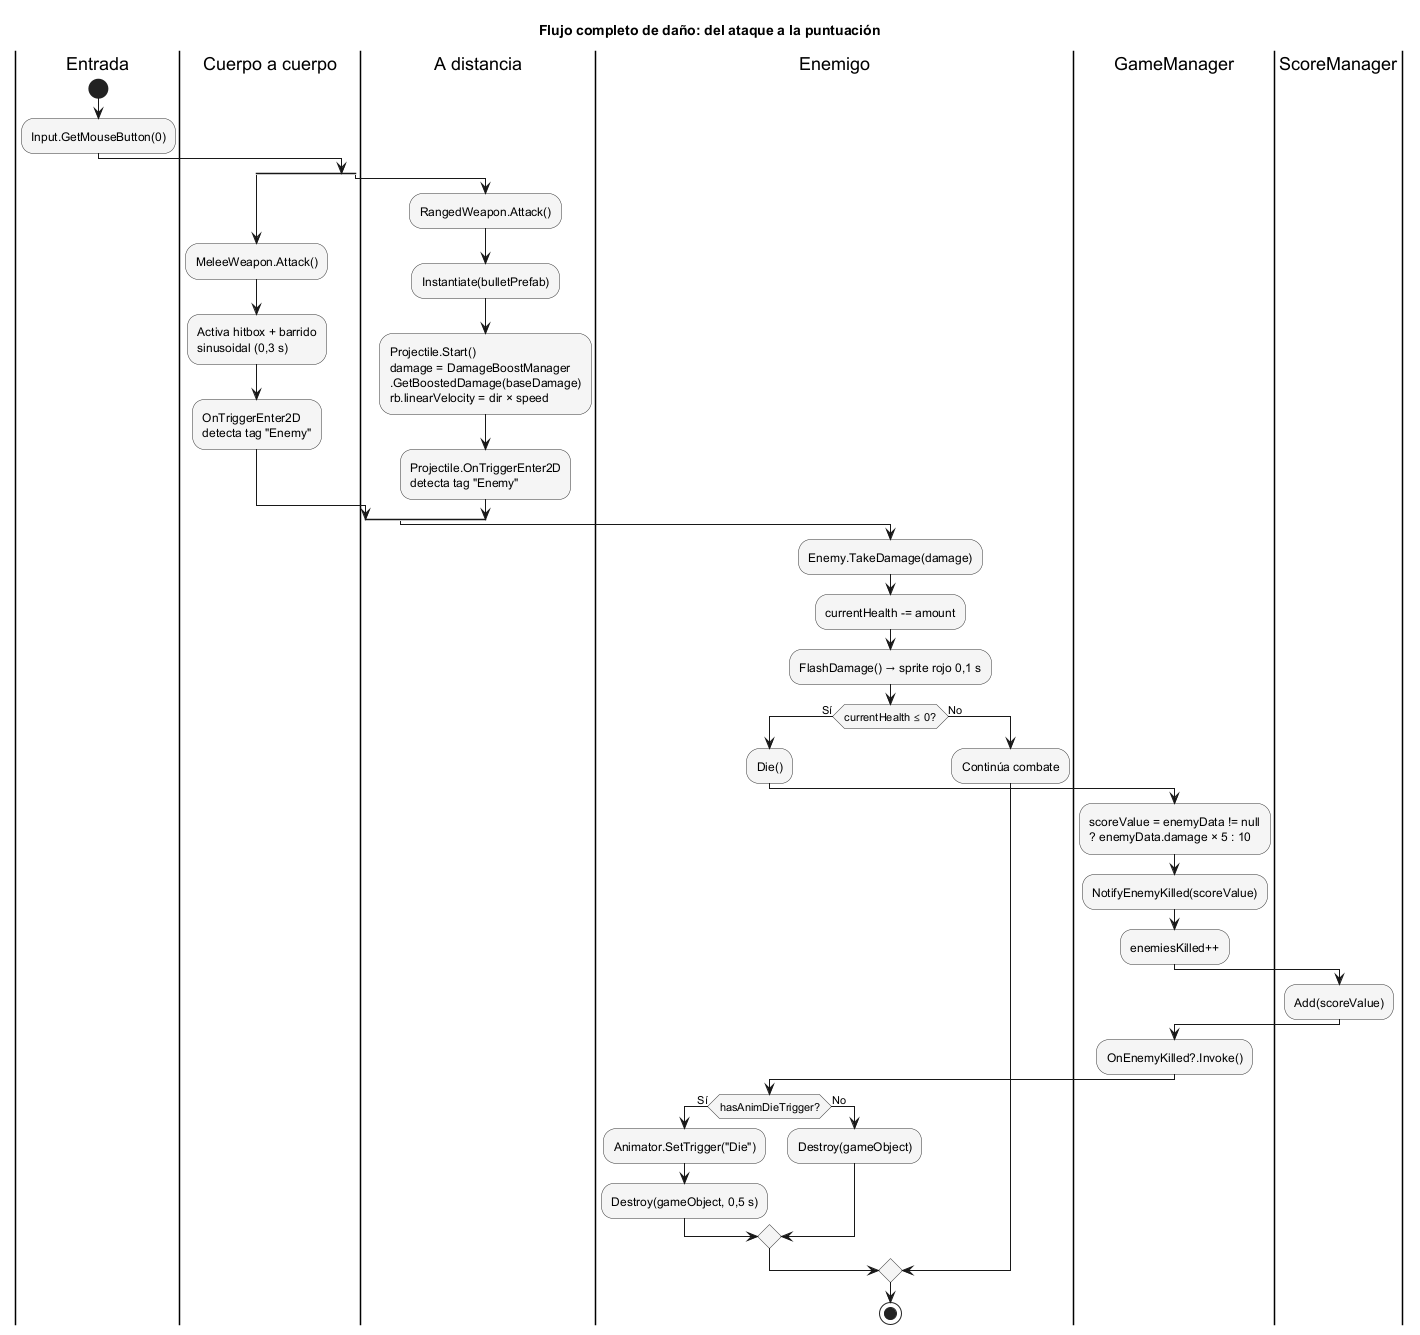
\includegraphics[width=0.95\textwidth,height=0.72\textheight,keepaspectratio]{Figuras/flujo_dano_completo.png}
\caption{
Diagrama de flujo del sistema de daño. \textit{Elaboración propia.}
}
\label{fig:placeholder-16}
\end{center}
\end{figure}
\vspace{-0.5em}

Este flujo evidencia la separación de responsabilidades aplicada: cada componente ejecuta exclusivamente su tarea (el arma ataca, el enemigo recibe daño, el gestor contabiliza) y la comunicación entre capas se realiza mediante invocaciones directas tipadas y eventos del patrón \textit{Observer}. La alternativa -- que el arma calculase ella misma la puntuación, o que el enemigo accediese directamente al marcador de la UI -- habría introducido dependencias transversales entre subsistemas que no comparten responsabilidad.
\vspace{-0.5em}
\begin{figure}[H]
\begin{center}
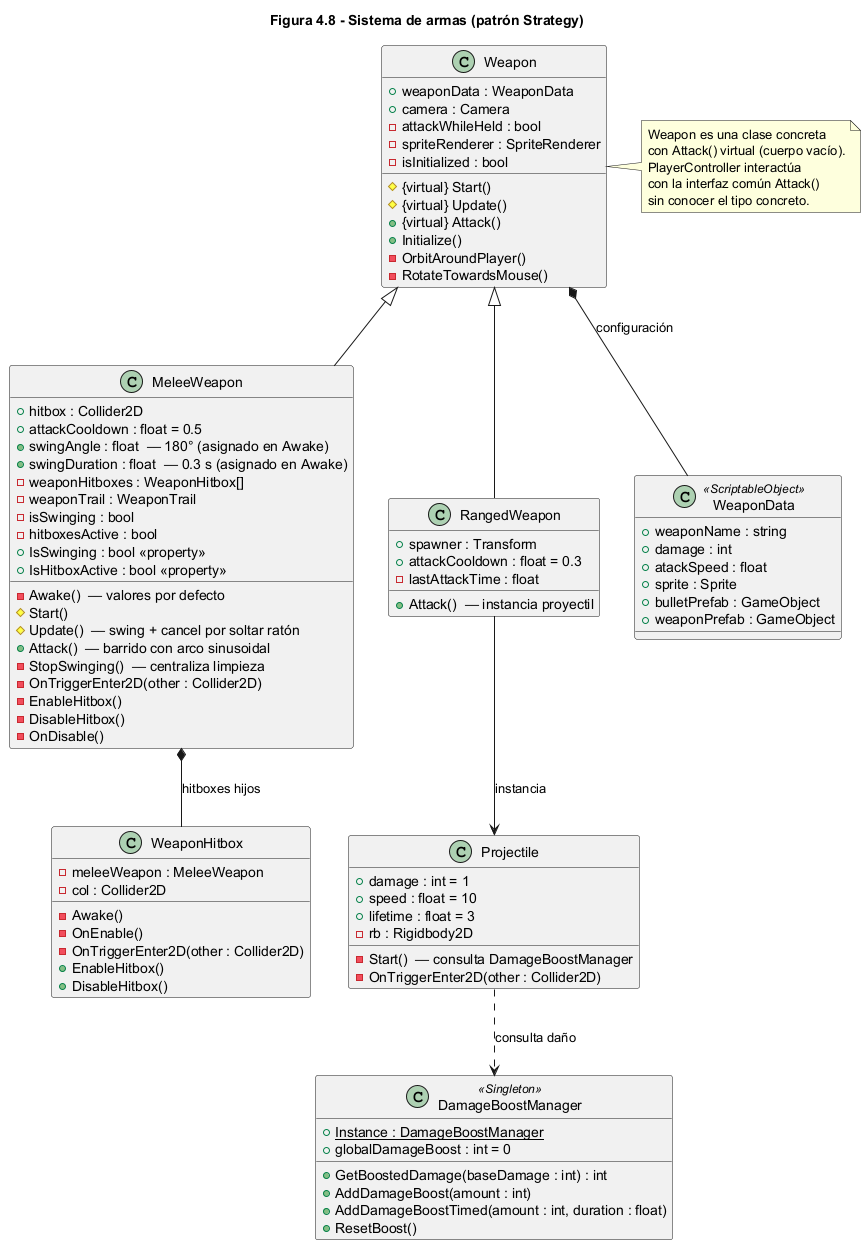
\includegraphics[width=0.95\textwidth,height=0.72\textheight,keepaspectratio]{Figuras/figura4_8_clases_armas.png}
\caption{
Diagrama de clases UML del sistema de armas. \textit{Elaboración propia.}
}
\label{fig:placeholder-17}
\end{center}
\end{figure}


\section{Sistema de generación procedural}


\textbf{Evolución iterativa.} La generación procedural fue el subsistema con mayor impacto arquitectónico derivado de la iteración. El diseño inicial cargaba una nueva escena de Unity para cada sala, lo que provocaba tiempos de carga de 0,5 a 1,5 segundos que rompían el ritmo de juego. El rediseño hacia la regeneración del \textit{tilemap} dentro de la misma escena (\texttt{RegenerateFloorKeepWalls}) eliminó estos tiempos de carga y modificó las responsabilidades del \texttt{RoomFlowController}. Adicionalmente, la distribución de tiles especiales evolucionó de una colocación puramente aleatoria (tile a tile) a un sistema de \textit{clusters} por expansión radial: la distribución aleatoria producía tiles aislados cuyo efecto era imperceptible durante el juego, mientras que los \textit{clusters} de 4-9 tiles generan zonas tácticas significativas que el jugador puede utilizar o evitar de forma deliberada.

\subsection{RoomGenerator: generación de salas}


El \texttt{RoomGenerator} constituye uno de los componentes de mayor complejidad del proyecto. Es responsable de la generación procedural de las salas del juego, incluyendo la estructura de muros, la distribución de tiles de suelo con variantes visuales y la colocación de tiles especiales con efectos.

Se seleccionó un enfoque de rejilla rectangular fija frente a alternativas más sofisticadas como BSP (\textit{Binary Space Partitioning}) o WFC (\textit{Wave Function Collapse}) por tres razones que afectan directamente a la jugabilidad y la complejidad de implementación:

\begin{enumerate}
\item \textbf{Simplicidad de posicionamiento de enemigos.} Con una rejilla rectangular fija de límites conocidos, cualquier coordenada dentro del perímetro de muros constituye una posición válida para la aparición de enemigos. Con BSP, las salas tendrían formas irregulares conectadas por pasillos estrechos, lo que requeriría verificaciones adicionales de accesibilidad y de línea de visión entre el jugador y el punto de aparición.
\item \textbf{Contención automática.} Los bordes perimetrales de muros generan colisionadores automáticos mediante el \texttt{TilemapCollider2D}, impidiendo que el jugador abandone el área de juego sin lógica de contención adicional.
\item \textbf{Variabilidad táctica mediante tiles.} La variabilidad entre salas no reside en la forma geométrica del espacio, sino en la distribución de tiles especiales dentro de él. Este enfoque combina la previsibilidad estructural (el jugador siempre sabe el tamaño de la sala) con la imprevisibilidad táctica (la ubicación de zonas de hielo, lodo y potenciación cambia en cada sala).
\end{enumerate}

\textbf{Configuración de la sala.} Cada sala se genera sobre una rejilla de $26 \times 12$ tiles, con un borde perimetral de muros de 1 tile de grosor:

\begin{lstlisting}
[SerializeField] private int roomWidth = 26;
[SerializeField] private int roomHeight = 12;
[SerializeField] private int wallBorderThicknessTiles = 1;
\end{lstlisting}


\textbf{Algoritmo de generación.} El proceso de generación de una sala sigue una secuencia de cinco pasos. A continuación se muestra la estructura real del método \texttt{GenerateRoom()} de \texttt{RoomGenerator.cs}, simplificada para mayor claridad:

\begin{lstlisting}
public void GenerateRoom() {
    // 1. Limpiar tilemaps anteriores
    if (clearWalls) wallTilemap.ClearAllTiles();
    floorTilemap.ClearAllTiles();

    // 2. Rellenar suelo y colocar tiles especiales en clusters
    for (int x = 0; x < roomWidth; x++)
        for (int y = 0; y < roomHeight; y++)
            floorTilemap.SetTile(pos, GetRandomNormalFloorTile());
    PlaceSpecialTilesClustered();   // hielo, lodo, curacion, potenciacion

    // 3. Colocar escaleras (en cada sala, en posicion aleatoria con margen)
    PlaceStairsTile();

    // 4. Generar borde de muros perimetrales (bucles inline)
    // wallTilemap.SetTile(...) en cada posicion del perimetro

    // 5. Actualizar colisionadores
    RefreshWallColliders();
    EnsureBoundaryCollidersSetup();
}
\end{lstlisting}


\textbf{Paso 1: Limpieza.} Se eliminan todos los tiles existentes en ambos \textit{tilemaps} (muros y suelo) mediante \texttt{wallTilemap.ClearAllTiles()} y \texttt{floorTilemap.ClearAllTiles()}, preparando la rejilla para una nueva generación.

\textbf{Paso 2: Generación de suelo con clusters.} Este paso constituye el núcleo del algoritmo de generación procedural. Primero se rellena toda la superficie interior con tiles normales seleccionados aleatoriamente entre las variantes disponibles. A continuación, se aplica el algoritmo de expansión por \textit{clusters} para colocar los tiles especiales.

\textbf{Algoritmo de expansión por \textit{clusters}.} Los tiles de hielo y lodo se distribuyen en manchas orgánicas de entre 4 y 9 tiles, generadas mediante un algoritmo de expansión por adyacencia de 4 direcciones desde un centro aleatorio. El método \texttt{PaintCluster} implementa esta lógica:

\begin{lstlisting}
private void PaintCluster(Vector2Int center, int targetCount, int maxRadius,
                          TileBase tile, HashSet<Vector2Int> reserved, int padding) {
    int minX = padding;
    int maxX = roomWidth - 1 - padding;
    int minY = padding;
    int maxY = roomHeight - 1 - padding;
    
    bool InBounds(Vector2Int c) =>
        c.x >= minX && c.x <= maxX && c.y >= minY && c.y <= maxY;
    int Manhattan(Vector2Int a, Vector2Int b) =>
        Mathf.Abs(a.x - b.x) + Mathf.Abs(a.y - b.y);
    
    var painted = new List<Vector2Int>(targetCount);
    if (InBounds(center) && reserved.Add(center)) {
        painted.Add(center);
        floorTilemap.SetTile(new Vector3Int(center.x, center.y, 0) + roomOffset, tile);
    }
    
    Vector2Int[] dirs = { Vector2Int.right, Vector2Int.left,
                          Vector2Int.up, Vector2Int.down };
    int safety = 200;
    while (painted.Count < targetCount && safety-- > 0) {
        if (painted.Count == 0) break;
        var baseCell = painted[Random.Range(0, painted.Count)];
        var next = baseCell + dirs[Random.Range(0, dirs.Length)];
        
        if (!InBounds(next)) continue;
        if (Manhattan(next, center) > maxRadius) continue;
        if (!reserved.Add(next)) continue;
        
        painted.Add(next);
        floorTilemap.SetTile(new Vector3Int(next.x, next.y, 0) + roomOffset, tile);
    }
}
\end{lstlisting}


El algoritmo comienza seleccionando una posición aleatoria como centro del \textit{cluster}. A continuación, expande el \textit{cluster} seleccionando en cada iteración una celda pintada al azar y desplazándose en una de las cuatro direcciones cardinales. La función local \texttt{InBounds} verifica que la posición candidata se encuentra dentro del margen útil del suelo (excluyendo un borde de \texttt{padding} celdas), y el \texttt{HashSet<Vector2Int> reserved} impide que una misma celda se pinte dos veces o sea reclamada por \textit{clusters} diferentes. La restricción de distancia Manhattan respecto al centro garantiza que el \textit{cluster} no se extienda más allá del radio máximo, produciendo manchas compactas de forma irregular y orgánica.


Este \textit{pipeline} se ejecuta también -- con una variante -- cuando el jugador avanza a la siguiente sala dentro de la misma escena: \texttt{RegenerateFloorKeepWalls()} omite los pasos 4 y 5 (los muros perimetrales no cambian) y únicamente regenera el suelo, los tiles especiales y las escaleras, reduciendo el coste computacional de la transición.

\textbf{Probabilidades de aparición de tiles especiales:}
\vspace{-0.5em}
\begin{table}[H]
\begin{center}
\small
\begin{tabular}{|p{0.22\textwidth}|p{0.18\textwidth}|p{0.25\textwidth}|p{0.18\textwidth}|}
\hline
\textbf{Tipo de tile} & \textbf{Probabilidad} & \textbf{Formato} & \textbf{Cantidad por sala} \\ \hline
Curación (\textit{Heal}) & 2 \% & Tile individual & Máximo 1 \\ \hline
Hielo (\textit{Ice}) & 12 \% & Cluster de 4-9 tiles & Variable \\ \hline
Lodo (\textit{Mud}) & 12 \% & Cluster de 4-9 tiles & Variable \\ \hline
Potenciación (\textit{PowerUp}) & 18 \% & Tile individual & 1-2 \\ \hline
\end{tabular}
\label{tab:probabilidades-tiles}
\end{center}
\end{table}
\TablaTitulo{Probabilidades y formato de distribución de tiles especiales.}
\vspace{-0.5em}

\begin{figure}[H]
\begin{center}
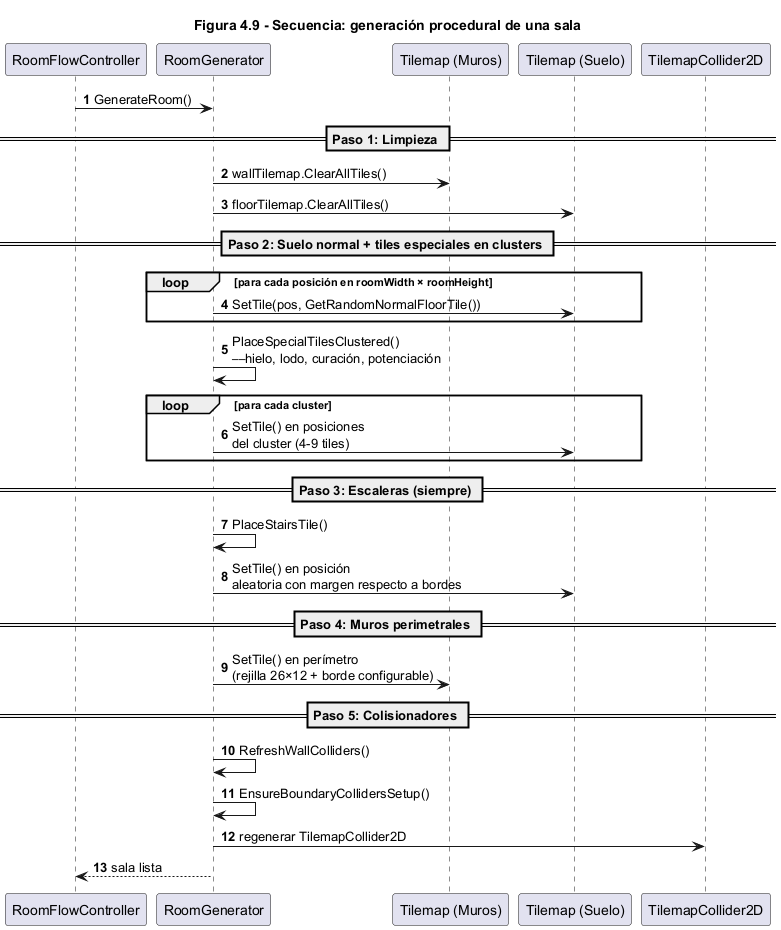
\includegraphics[width=0.95\textwidth,height=0.72\textheight,keepaspectratio]{Figuras/figura4_9_secuencia_generacion_sala.png}
\caption{
Diagrama de secuencia UML de la generación procedural de una sala. \textit{Elaboración propia.}
}
\label{fig:placeholder-19}
\end{center}
\end{figure}

\textbf{Paso 3: Colocación de escaleras.} Las escaleras se colocan en cada sala generada, en una posición aleatoria dentro de una zona segura definida por \texttt{stairsPaddingTiles} (margen configurable respecto a los bordes). El método \texttt{PlaceStairsTile()} aplica el margen sobre el rango de la rejilla y selecciona un punto aleatorio con \texttt{Random.Range}; si el padding es mayor que el espacio disponible, usa el centro como posición de respaldo. Las escaleras permanecen visibles desde el primer momento, pero el jugador no puede interactuar con ellas hasta que la sala se completa.

\textbf{Paso 4: Generación de muros perimetrales.} Se itera sobre las posiciones del perímetro de la rejilla y se coloca un tile de muro en cada posición mediante \texttt{wallTilemap.SetTile()}, creando un recinto cerrado con colisionadores automáticos. El grosor del borde es configurable mediante \texttt{wallBorderThicknessTiles}.

\textbf{Paso 5: Actualización de colisionadores.} Se refresca el \texttt{TilemapCollider2D} de los muros mediante \texttt{RefreshWallColliders()}, y se garantiza la contención del jugador mediante \texttt{EnsureBoundaryCollidersSetup()}, que mantiene \texttt{BoxCollider2D} adicionales en los cuatro bordes como respaldo.

\subsection{VariantTile: tiles con variantes visuales y selección determinista}


La clase \texttt{VariantTile} extiende \texttt{TileBase} de Unity para soportar múltiples sprites por tile, proporcionando variedad visual sin afectar a la jugabilidad. Se seleccionó un sistema de \textit{hash} determinista frente a la alternativa de selección aleatoria pura (\texttt{Random.Range}) porque esta última habría producido cambios visuales cada vez que el \textit{tilemap} se redibuja (por ejemplo, al redimensionar la ventana del editor o al ocultar y mostrar la cámara), generando un efecto de parpadeo visual perceptible por el jugador:

\begin{lstlisting}
public class VariantTile : TileBase {
    public Sprite[] variants;        // Array de variantes visuales para este tipo de tile
    public bool deterministic = true;
    public int seed = 1337;
    public TileEffect tileEffect;    // Efecto asociado (hielo, lodo, curacion, etc.)
    
    public override void GetTileData(Vector3Int position, ITilemap tilemap, 
                                      ref TileData tileData) {
        if (variants != null && variants.Length > 0) {
            int index;
            if (deterministic) {
                unchecked {
                    int hash = seed;
                    hash = hash * 31 + position.x;
                    hash = hash * 17 + position.y;
                    if (position.x != 0) hash ^= position.x << 2;
                    if (position.y != 0) hash ^= position.y << 5;
                    if (hash < 0) hash = -hash;
                    index = hash % variants.Length;
                }
            } else {
                index = Random.Range(0, variants.Length);
            }

            tileData.sprite = variants[index];
        }
    }
}
\end{lstlisting}


Línea por línea:

\begin{itemize}
\item \texttt{public Sprite[] variants}: array configurado desde el inspector de Unity que contiene las variantes visuales de un mismo tipo de tile.
\item \texttt{public bool deterministic}: habilita la selección determinista (estable) de sprite por posición. Si se desactiva, el sprite se selecciona de forma pseudoaleatoria, lo que puede producir variaciones visuales entre repintados.
\item \texttt{public int seed}: semilla adicional que permite variar la distribución sin perder determinismo.
\item \texttt{unchecked { ... }}: asegura que la aritmética de enteros permite desbordamientos sin lanzar excepciones, lo que se utiliza como parte de la mezcla del hash.
\item \texttt{hash = hash \textit{ 31 + position.x; hash = hash } 17 + position.y; ... index = hash \% variants.Length}: cálculo de un hash simple que mezcla la semilla y las coordenadas del tile para obtener un índice estable dentro del rango de variantes.
\end{itemize}

\subsection{TileEffect: efectos de tiles}


Los efectos de tiles se definen como \textit{ScriptableObjects}, lo que permite crear y configurar nuevos efectos desde el inspector de Unity sin modificar el código:

\begin{lstlisting}
[CreateAssetMenu(menuName = "Tiles/TileEffect")]
public class TileEffect : ScriptableObject {
    public string tileName;
    public TileEffectType effectType = TileEffectType.None;
    
    public int healthChange = 0;
    public float speedMultiplier = 1f;
    public float effectDuration = 0f;
    
    public float tickRate = 1f;
    public bool continuous = false;
    
    public Color tintColor = Color.white;
    public GameObject vfxPrefab;
}
\end{lstlisting}


La enumeración \texttt{TileEffectType} define los tipos de efecto posibles:

\begin{lstlisting}
public enum TileEffectType {
    None,       // Sin efecto
    Heal,       // Restaura vida
    Damage,     // Inflige dano
    SpeedUp,    // Incrementa velocidad
    SpeedDown,  // Reduce velocidad
    Ice,        // Tile de hielo
    Mud,        // Tile de lodo
    PowerUp     // Incrementa dano
}
\end{lstlisting}


\subsection{FloorTileManager: aplicación de efectos}


El \texttt{FloorTileManager} detecta sobre qué tile se encuentra el jugador en cada fotograma y aplica el efecto correspondiente:

\begin{lstlisting}
void Update() {
    if (floorTilemap == null || playerTransform == null) return;
    
    Vector3Int tilePos = floorTilemap.WorldToCell(playerTransform.position);
    
    if (tilePos != currentTilePos) {
        OnExitTile();
        currentTilePos = tilePos;
        OnEnterTile();
    }
    
    if (currentEffect?.continuous == true) {
        if (Time.time >= lastEffectTime + currentEffect.tickRate) {
            ApplyEffect(currentEffect);
            lastEffectTime = Time.time;
        }
    }
}
\end{lstlisting}


La conversión de la posición del jugador en coordenadas de mundo a coordenadas de tile se realiza mediante \texttt{WorldToCell}. Cuando el jugador cambia de tile, se ejecutan las funciones de salida del tile anterior y entrada al nuevo tile. Para los efectos con el indicador (\textit{flag}) \texttt{continuous} activado, el efecto se aplica periódicamente según la frecuencia definida en \texttt{tickRate}.

\textbf{Seguimiento visual de efectos.} Al instanciar los efectos visuales (VFX) de un tile, se añade el componente \texttt{VFXFollower} al objeto instanciado para que el efecto visual siga la posición de la entidad afectada (jugador o enemigo). Sin este componente, el VFX quedaría fijo en la posición de instanciación mientras la entidad se desplaza, produciendo una desincronización visual.

\textbf{Persistencia de efectos de velocidad.} Los efectos de modificación de velocidad (hielo, lodo) persisten durante un periodo configurable tras abandonar el tile, evitando que el efecto desaparezca bruscamente:

\begin{lstlisting}
private void ApplySpeedModifier(float multiplier) {
    if (playerController == null) return;
    playerController.SetSpeedMultiplier(multiplier);
    hasSpeedModifier = true;
}

private IEnumerator RemoveSpeedAfterDelay(float seconds) {
    yield return new WaitForSeconds(seconds);
    
    if (hasSpeedModifier && playerController != null) {
        playerController.ResetSpeed();
        hasSpeedModifier = false;
    }
}
\end{lstlisting}


La separación de responsabilidades es deliberada: \texttt{ApplySpeedModifier} solo aplica el multiplicador al controlador del jugador, mientras que la persistencia del efecto tras abandonar el tile se gestiona en el bloque \texttt{ApplyEffect()}, donde se lanza la corutina \texttt{RemoveSpeedAfterDelay(persistEffectSeconds)} si el tiempo de persistencia es mayor que cero.

\textbf{Integración con enemigos.} Los efectos de velocidad de los tiles también se aplican a los enemigos mediante el componente \texttt{EnemyTileEffectReceiver}, que se añade automáticamente a cada enemigo al ser instanciado por el \texttt{EnemyManager}. Este componente consulta el tile sobre el que se encuentra el enemigo y aplica el multiplicador de velocidad correspondiente a través de \texttt{Enemy.SetTileSpeedMultiplier()}, lo que permite al jugador utilizar estas zonas de forma estratégica.

\subsection{DamageBoostManager: bonificación de daño}


El \texttt{DamageBoostManager} gestiona las bonificaciones de daño otorgadas por los tiles de potenciación. Implementa el patrón \textit{Singleton} y soporta bonificaciones permanentes y temporales:

\begin{lstlisting}
public void AddDamageBoostTimed(int amount, float duration) {
    if (duration <= 0f) {
        AddDamageBoost(amount);  // Permanente
        return;
    }
    
    AddDamageBoost(amount);
    StartCoroutine(RemoveDamageBoostAfterDelay(amount, duration));
}

public int GetBoostedDamage(int baseDamage) {
    return baseDamage + globalDamageBoost;
}
\end{lstlisting}


Los proyectiles consultan al \texttt{DamageBoostManager} en su inicialización para calcular su daño efectivo, lo que permite que la bonificación se aplique de forma global y coherente a todas las fuentes de daño del jugador.



\section{Sistema de gestión de salas}


\textbf{Evolución iterativa.} El sistema de gestión de salas se vio directamente afectado por el rediseño de la generación procedural. Cuando cada sala era una escena independiente, el \texttt{RoomController} no existía como tal: la lógica de escaleras y progresión residía en scripts de cada escena. Al consolidar todo el juego en una única escena, se creó el \texttt{RoomController} como componente central para gestionar la detección de entrada del jugador, el bloqueo de escaleras durante el combate y la detección de sala completada.

\subsection{RoomController: control de sala individual}


El \texttt{RoomController} gestiona el ciclo de vida de una sala individual: la detección de entrada del jugador, la activación de la aparición de enemigos, el bloqueo de escaleras durante el combate y la detección de sala completada.

\begin{lstlisting}
void OnTriggerEnter2D(Collider2D other) {
    if (other.CompareTag("Player")) {
        playerInside = true;
        
        if (!isCleared) {
            CloseAllDoors();
        }
    }
}
\end{lstlisting}


Al detectar la entrada del jugador mediante el sistema de \textit{triggers} de Unity, el controlador bloquea las escaleras de la sala y activa la aparición de enemigos. Las escaleras permanecen bloqueadas hasta que todos los enemigos han sido eliminados, momento en el cual se habilitan automáticamente para permitir la progresión.

\begin{figure}[H]
\begin{center}
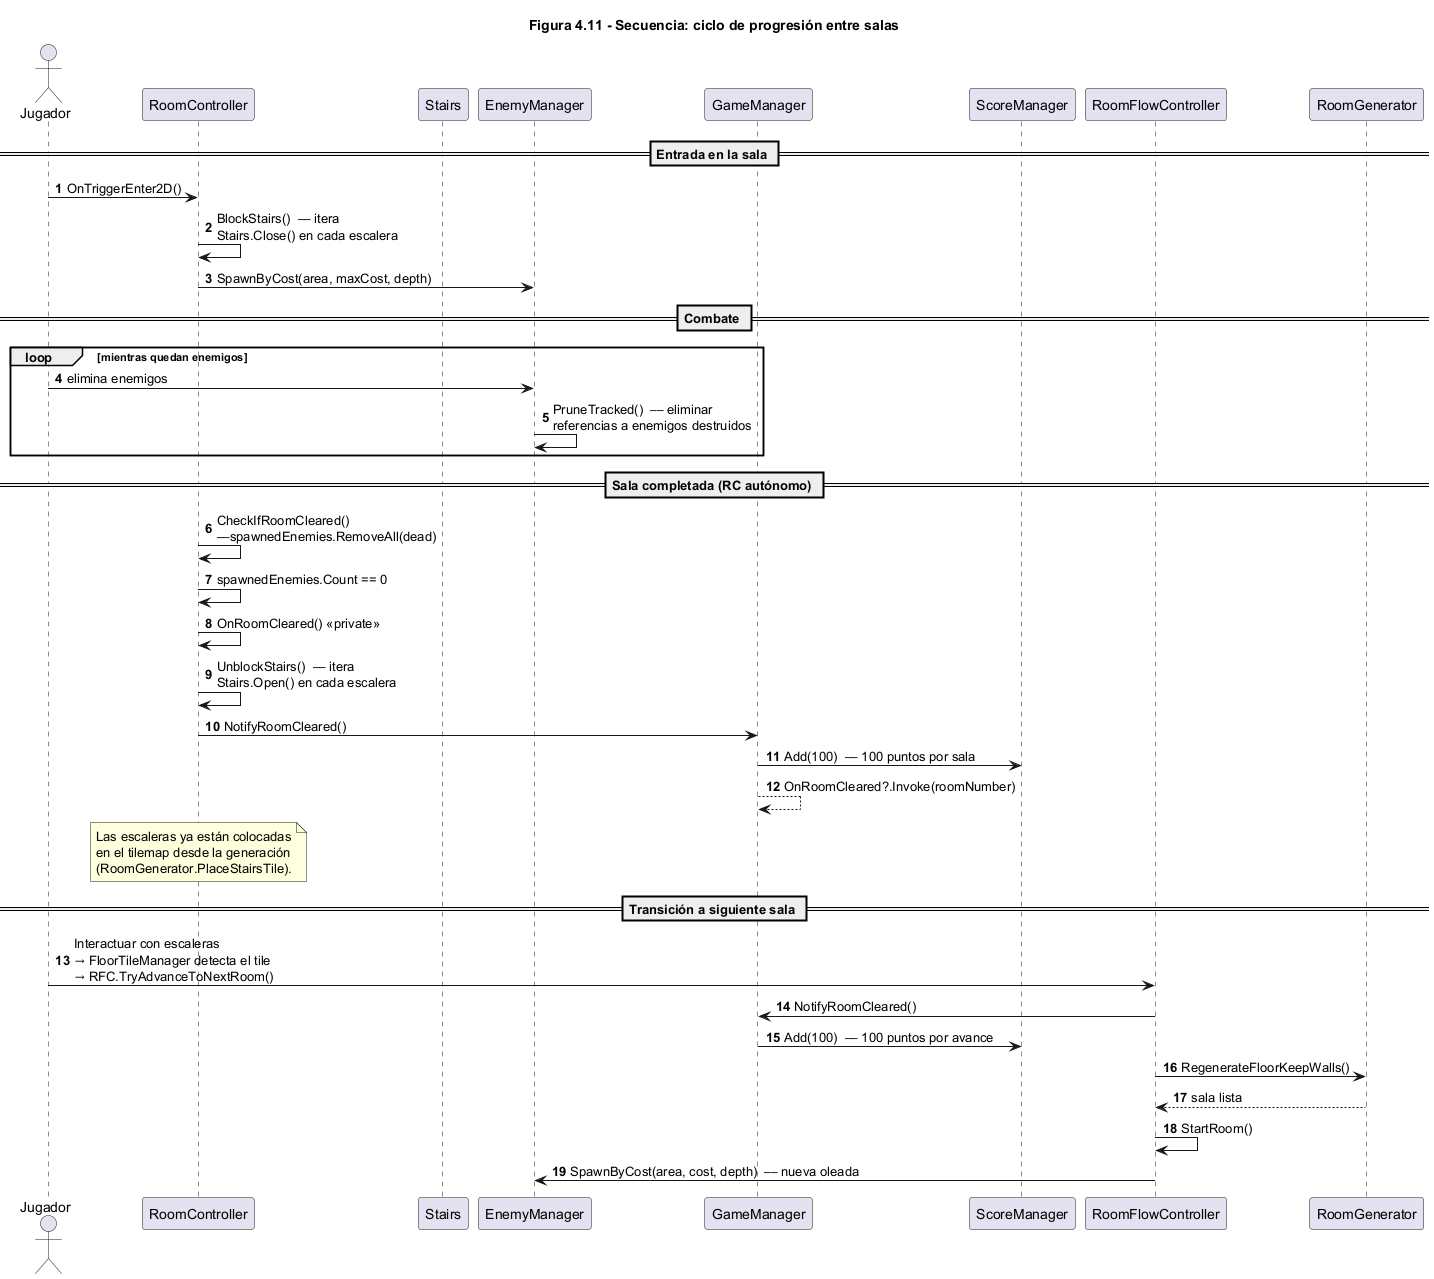
\includegraphics[width=0.95\textwidth,height=0.72\textheight,keepaspectratio]{Figuras/figura4_11_secuencia_progresion_salas.png}
\caption{
Diagrama de secuencia UML del ciclo de progresión entre salas. \textit{Elaboración propia.}
}
\label{fig:placeholder-21}
\end{center}
\end{figure}


\subsection{Stairs: lógica de escaleras}


El componente de escaleras (implementado como clase \texttt{Door} por cuestiones de diseño) gestiona el estado visual y funcional de acceso:

\begin{lstlisting}
public void Open(bool playEffects = true) {
    if (isOpen) return;
    isOpen = true;
    doorCollider.enabled = false;
}

public void Close(bool playEffects = true) {
    isOpen = false;
    doorCollider.enabled = true;
}
\end{lstlisting}


La escalera alterna entre un estado bloqueado y un estado habilitado.



\section{Sistema de interfaz de usuario}


\textbf{Evolución iterativa.} La interfaz de usuario fue el último subsistema en integrarse con el patrón \textit{Observer}. En las primeras iteraciones, cada componente de UI consultaba directamente al \texttt{GameManager} en su método \texttt{Update()} (lectura síncrona por sondeo), lo que generaba comprobaciones redundantes en cada fotograma y acoplaba la interfaz con la implementación interna del gestor. La adopción del patrón \textit{Observer} -- suscripción al evento \texttt{OnGameStateChanged} -- eliminó esta dependencia: los paneles de pausa, derrota y victoria solo ejecutan lógica cuando reciben una notificación de cambio de estado, no en cada fotograma. El sistema de corazones evolucionó de una implementación estática (número fijo de corazones en la escena) a una generación dinámica basada en \texttt{maxHealth}, lo que permitió que las clases de personaje con distinta cantidad de vida máxima se representasen correctamente sin configuración manual.

\subsection{HeartDisplay: representación de vida}


El \texttt{HeartDisplay} proporciona una representación visual dinámica de la vida del jugador mediante iconos de corazones. El sistema crea los corazones de forma dinámica en función de la vida máxima del personaje:

\begin{lstlisting}
public void InitializeHearts(int maxHealth) {
    ClearHearts();
    maxHearts = Mathf.Max(0, maxHealth);
    
    for (int i = 0; i < maxHearts; i++) {
        CreateHeart(i);
    }
}
\end{lstlisting}


La actualización responde a los cambios en la vida del jugador, alternando los sprites de corazón lleno y vacío:

\begin{lstlisting}
public void UpdateHearts(int currentHealth) {
    int clampedHealth = Mathf.Clamp(currentHealth, 0, maxHearts);
    
    for (int i = 0; i < heartImages.Count; i++) {
        Image heartImage = heartImages[i];
        if (heartImage == null) continue;
        
        heartImage.sprite = i < clampedHealth ? heartFull : heartEmpty;
        heartImage.enabled = true;
    }
}
\end{lstlisting}


\subsection{PauseMenu: menú de pausa}


El \texttt{PauseMenu} se suscribe al evento \texttt{OnGameStateChanged} del \texttt{GameManager} y activa o desactiva su panel según el estado actual del juego:

\begin{lstlisting}
void Start() {
    EnsureRuntimeUIIfMissing();
    WireButtonsOnce();
    
    if (pauseMenuPanel != null)
        pauseMenuPanel.SetActive(false);
    
    GameManager.OnGameStateChanged += OnGameStateChanged;
}

private void OnGameStateChanged(GameState newState) {
    EnsureRuntimeUIIfMissing();
    if (pauseMenuPanel == null) return;
    
    bool shouldShow = (newState == GameState.Paused);
    pauseMenuPanel.SetActive(shouldShow);
}
\end{lstlisting}


Este diseño ejemplifica la aplicación del patrón \textit{Observer}: el menú de pausa no consulta activamente el estado del juego, sino que reacciona a la notificación de cambio de estado emitida por el \texttt{GameManager}. Las llamadas a \texttt{EnsureRuntimeUIIfMissing()} y \texttt{WireButtonsOnce()} garantizan que la interfaz de pausa exista y tenga sus botones configurados incluso cuando el \texttt{PauseMenu} se crea en tiempo de ejecución sin referencias previas asignadas en el inspector. Esto permite añadir o eliminar elementos de interfaz reactivos sin modificar el código del gestor central.

\subsection{Pantallas de fin de partida}


Las pantallas de derrota (\texttt{GameOverScreen}) y victoria (\texttt{VictoryScreen}) se activan automáticamente al cambiar el estado del juego a \texttt{GameOver} o \texttt{Victory}, respectivamente:

\begin{lstlisting}
public void Show() {
    if (victoryPanel == null) return;
    victoryPanel.SetActive(true);
    
    if (scoreText != null && ScoreManager.Instance != null)
        scoreText.text = $"Puntuacion Final: {ScoreManager.Instance.CurrentScore}";
    if (roomsClearedText != null && GameManager.Instance != null)
        roomsClearedText.text = $"Salas limpiadas: {GameManager.Instance.RoomsCleared}";
    if (enemiesKilledText != null && GameManager.Instance != null)
        enemiesKilledText.text = $"Enemigos eliminados: {GameManager.Instance.EnemiesKilled}";
    if (timeText != null) {
        float runTime = Time.time - runStartTime;
        int minutes = Mathf.FloorToInt(runTime / 60f);
        int seconds = Mathf.FloorToInt(runTime % 60f);
        timeText.text = $"Tiempo: {minutes:00}:{seconds:00}";
    }
}
\end{lstlisting}


Ambas pantallas muestran un texto que representa el final de la partida y redirigen al menú principal tras un tiempo.


\begin{figure}[H]
\begin{center}
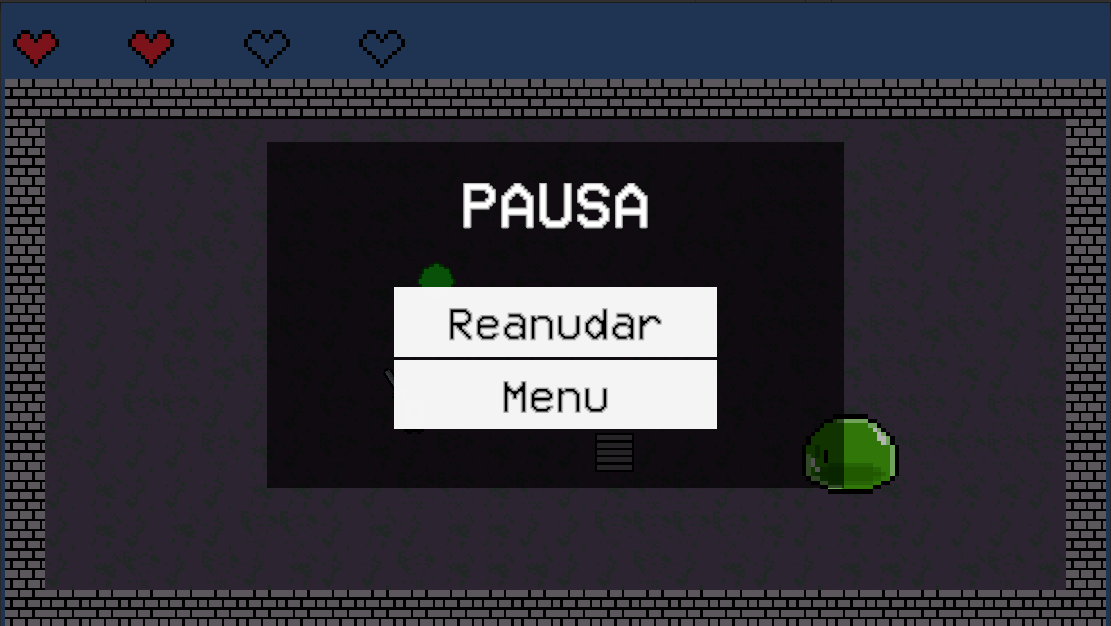
\includegraphics[width=0.9\textwidth]{Figuras/captura_14.png}
\caption{Captura de pantalla del menú de pausa de \textit{Ascension}, mostrando las opciones de reanudar y menú principal. \textit{Elaboración propia.}}
\label{fig:placeholder-23}
\end{center}
\end{figure}

\subsection{ScoreboardMenuUI: historial de puntuaciones}


El historial de puntuaciones se genera dinámicamente a partir de los datos almacenados por el \texttt{ScoreManager}. En lugar de instanciar un \textit{prefab} por cada entrada, el componente utiliza un único campo \texttt{TextMeshProUGUI} -- un sistema de renderizado de texto de alta calidad integrado en Unity que soporta formato enriquecido, sombreado y alineación precisa a nivel de píxel -- y construye todo el listado mediante un \texttt{StringBuilder}, lo que resulta más eficiente en memoria y evita la necesidad de gestionar la destrucción de objetos instanciados:

\begin{lstlisting}
public void Refresh() {
    if (listText == null) return;
    
    var sb = new StringBuilder();
    var entries = ScoreManager.Instance != null
                     ? ScoreManager.Instance.GetHistory() : null;
    
    sb.AppendLine("SCORES");
    sb.AppendLine("------");
    
    if (entries == null || entries.Count == 0) {
        sb.AppendLine("(sin partidas guardadas)");
        listText.text = sb.ToString();
        return;
    }
    
    int rank = 1;
    foreach (var e in entries) {
        sb.Append(rank).Append(". ")
          .Append(e.score).Append(" pts")
          .Append(" | ").Append(e.result)
          .Append(" | ").Append(e.playerClass)
          .Append(" | R ").Append(e.roomsCleared)
          .Append(" | K ").Append(e.enemiesKilled)
          .AppendLine();
        rank++;
    }
    
    listText.text = sb.ToString();
}
\end{lstlisting}




\section{Sistemas preparados para extensión}


\textbf{Evolución iterativa.} Ambos sistemas descritos en esta sección (jefes con fases y generación procedural de armas) se desarrollaron como prototipos funcionales durante iteraciones intermedias del proyecto. La decisión de no integrarlos en el bucle de juego final se tomó tras evaluar la prioridad de las tareas restantes: el equilibrado de dificultad de los jefes con fases múltiples y la interfaz de recogida de armas generadas requerían un volumen de trabajo que habría comprometido la entrega de los subsistemas prioritarios. Se optó por mantener el código desarrollado como extensión documentada, alineándose con el principio de apertura-cierre: la arquitectura permite su integración futura sin modificar los subsistemas existentes.

La arquitectura del proyecto se ha diseñado teniendo en cuenta la extensibilidad. Se han desarrollado dos sistemas cuya estructura se ha preparado a nivel de código pero que no se encuentran completamente integrados en el bucle de juego al cierre del presente trabajo:

\subsection{Sistema de jefes con fases múltiples}


Se ha desarrollado el componente \texttt{BossController} que implementa un sistema de jefes con dos fases diferenciadas basadas en el porcentaje de vida restante. El diseño contempla la transición automática a la segunda fase al alcanzar el 50 \% de vida, con cambios en la cadencia de ataque, la velocidad de movimiento y los patrones de disparo. No obstante, al no encontrarse integrado en el bucle de progresión de salas, su funcionamiento en una partida completa no se ha verificado de forma consistente; su integración requiere trabajo adicional en el equilibrado de dificultad y en la definición de patrones de ataque más variados.

\subsection{Generación procedural de armas con rareza}


Se ha desarrollado el componente \texttt{WeaponGenerator} que implementa un sistema de generación procedural de armas con cuatro niveles de rareza (Común, Poco Común, Raro, Legendario) y escalado de estadísticas basado en la profundidad de la mazmorra. Al no encontrarse integrado en el flujo de juego -- aparición de armas como objetos recogibles en las salas --, su funcionamiento en una partida completa no se ha verificado de forma consistente; la integración constituye un desarrollo pendiente para futuras iteraciones del proyecto.

Estos dos sistemas se analizan con mayor detalle en el apartado de líneas de trabajo futuro.



\section{Compilación y ejecución}


\textbf{Evolución iterativa.} Las primeras versiones del proyecto se ejecutaban exclusivamente desde el editor de Unity durante el desarrollo. La generación del ejecutable final se realizó una vez estabilizados los subsistemas principales, verificando que el comportamiento del juego compilado fuese idéntico al observado en el editor.

\subsection{Proceso de compilación}


La compilación del proyecto se realiza desde la ventana \textit{Build Profiles} del editor de Unity (\texttt{File > Build Profiles}). La configuración utilizada es la siguiente:

\begin{itemize}
\item \textbf{Motor:} Unity 6 (versión 6000.2.7f2).
\item \textbf{Plataforma objetivo:} Windows, arquitectura Intel 64-bit.
\item \textbf{Backend de scripting:} Mono (compatible con .NET Standard 2.1).
\item \textbf{Escenas incluidas en el \textit{build}:} se incluyen las tres escenas del proyecto en el orden definido por el flujo de juego:
\end{itemize}

\begin{enumerate}
\item \texttt{Scenes/MainMenu} (índice 0) -- menú principal.
\item \texttt{Scenes/ClassSelection} (índice 1) -- pantalla de selección de clase.
\item \texttt{Scenes/GameScene} (índice 2) -- escena principal de juego.
\end{enumerate}

\begin{itemize}
\item \textbf{Opciones de compilación desactivadas:} \textit{Copy PDB files}, \textit{Create Visual Studio Solution} y \textit{Development Build}. Esto genera un ejecutable de producción optimizado, sin símbolos de depuración ni herramientas de \textit{profiling}.
\end{itemize}

El orden de las escenas es relevante: Unity carga automáticamente la escena con índice 0 al iniciar el ejecutable, por lo que \texttt{MainMenu} debe ocupar la primera posición para que el jugador acceda al menú principal al arrancar el juego.

Para generar el ejecutable, se selecciona la plataforma \textit{Windows} en la ventana \textit{Build Profiles}, se verifica que las tres escenas estén incluidas y ordenadas correctamente, y se pulsa \textit{Build}. Unity compila los scripts de C\# mediante el compilador Roslyn integrado, empaqueta los activos del proyecto (sprites, tilemaps, prefabs, ScriptableObjects) en archivos binarios optimizados y genera el ejecutable junto con sus dependencias.

\subsection{Estructura del ejecutable}


El proceso de compilación genera la siguiente estructura de archivos en el directorio de salida:

\begin{lstlisting}
Build/
 Ascension.exe                           Ejecutable principal
 UnityPlayer.dll                         Motor de ejecucion de Unity
 UnityCrashHandler64.exe                 Gestor de errores criticos
 Ascension_Data/                         Activos compilados del proyecto
    level0, level1, level2              Escenas empaquetadas
    resources.assets                    Activos marcados como Resources
    sharedassets02.assets              Activos especificos de cada escena
    globalgamemanagers                  Configuracion global del proyecto
    Managed/                            Ensamblados .NET compilados
    Plugins/x86_64/                     Bibliotecas nativas
 MonoBleedingEdge/                       Runtime de Mono (.NET)
 D3D12/                                  Bibliotecas de renderizado DirectX 12
\end{lstlisting}


Los archivos \texttt{level0}, \texttt{level1} y \texttt{level2} corresponden a las tres escenas del proyecto en el orden definido en \textit{Build Profiles}. El directorio \texttt{Managed/} contiene los ensamblados compilados a partir de los scripts de C\# del proyecto (\texttt{Assembly-CSharp.dll}) y las bibliotecas del framework de Unity.

\subsection{Ejecución del juego}


Para ejecutar el juego, el usuario debe:

\begin{enumerate}
\item Copiar la carpeta \texttt{Build/} completa a la ubicación deseada, manteniendo la estructura de directorios intacta.
\item Ejecutar \texttt{Ascension.exe}.
\end{enumerate}

No es necesario instalar Unity ni ningún componente adicional: el ejecutable incluye el \textit{runtime} de Mono y las bibliotecas del motor de Unity necesarias para la ejecución autónoma. El juego se inicia mostrando la pantalla del menú principal, desde la cual el jugador puede acceder a la selección de clase, consultar el historial de puntuaciones o salir del juego.

\textbf{Requisitos mínimos del sistema:}

\begin{itemize}
\item Sistema operativo: Windows 10 (64 bits) o posterior.
\item Procesador: compatible con x86_64.
\item Memoria: 4 GB de RAM.
\item Gráficos: compatible con DirectX 11 o DirectX 12.
\item Almacenamiento: aproximadamente 100 MB de espacio en disco.
\end{itemize}
